%% =============================================================
%%  Neuroscience Informatics (Elsevier) -- NEURI-D-26-00184, revision 1
%%  Reconstructed editable source (see README_SOURCE.md): rebuilt from the
%%  authors' June 2026 LaTeX project; all tables, figures and numeric macros in
%%  tables/ and figures/ are regenerated by the analysis code (strokerev).
%%  Compile: pdflatex -> bibtex -> pdflatex x2
%% =============================================================
\documentclass[preprint,10pt]{elsarticle}

\usepackage[utf8]{inputenc}
\usepackage[T1]{fontenc}
\usepackage{lmodern}
\usepackage{amsmath,amssymb}
\usepackage{booktabs}
\usepackage{array}
\usepackage{graphicx}
\usepackage{float}
\usepackage{caption}
\usepackage[table]{xcolor}
\usepackage{geometry}
\usepackage[mathlines]{lineno}
\usepackage{hyperref}
\DeclareMathOperator*{\argmax}{arg\,max}
\DeclareMathOperator*{\argmin}{arg\,min}
\geometry{margin=2.5cm}
\hypersetup{hidelinks}
\captionsetup{font=small}

\newcommand{\Nreg}{1{,}653}
\newcommand{\Nrecon}{1{,}618}
\newcommand{\Nelig}{1{,}579}
\newcommand{\Nlab}{982}
\newcommand{\Ndeaths}{338}
\newcommand{\Nunres}{597}
\newcommand{\Mortlab}{34.4}
\newcommand{\MortlabLo}{31.5}
\newcommand{\MortlabHi}{37.4}
\newcommand{\NexBlank}{6}
\newcommand{\NexDate}{6}
\newcommand{\NexAge}{3}
\newcommand{\NexTIA}{24}
\newcommand{\NEone}{305}
\newcommand{\NEtwo}{33}
\newcommand{\NNone}{2}
\newcommand{\NNtwo}{617}
\newcommand{\NNthree}{5}
\newcommand{\NNfour}{20}
\newcommand{\NstrictLab}{949}
\newcommand{\NstrictDeaths}{305}
\newcommand{\Mortstrict}{32.1}
\newcommand{\BoundLo}{21.4}
\newcommand{\BoundHi}{59.2}
\newcommand{\Mortinhosp}{23.6}
\newcommand{\MortinhospLo}{21.4}
\newcommand{\MortinhospHi}{26.0}
\newcommand{\Ninhospden}{1{,}292}
\newcommand{\Mortipw}{27.5}
\newcommand{\MortipwLo}{25.0}
\newcommand{\MortipwHi}{30.1}
\newcommand{\Nipwpop}{1{,}456}
\newcommand{\Nnodisp}{123}
\newcommand{\IPWess}{830}
\newcommand{\IPWcap}{3.91}
\newcommand{\IPWmax}{8.9}
\newcommand{\IPWntrunc}{10}
\newcommand{\OrigObs}{803}
\newcommand{\OrigInf}{218}
\newcommand{\OrigUnl}{594}
\newcommand{\OrigLab}{1{,}021}
\newcommand{\OrigDeaths}{345}
\newcommand{\OrigMort}{33.8}
\newcommand{\OrigObsDeaths}{162}
\newcommand{\DeltaMARearly}{30.7}
\newcommand{\DeltaMARper}{29.8}
\newcommand{\DeltaMin}{26.6}
\newcommand{\DeltaMax}{41.7}
\newcommand{\DeltaTwoEarly}{33.4}
\newcommand{\DeltaFourEarly}{37.1}
\newcommand{\PDearlyK}{27}
\newcommand{\PDearlyN}{358}
\newcommand{\PDearly}{7.5}
\newcommand{\PDlateK}{4}
\newcommand{\PDlateN}{241}
\newcommand{\PDlate}{1.7}
\newcommand{\IHDeathOneEarly}{80/83}
\newcommand{\IHDeathOneLate}{3/172}
\newcommand{\DispMissTwenty}{107}
\newcommand{\AdmTwenty}{191}
\newcommand{\OtherLate}{132}
\newcommand{\AdmLate}{205}
\newcommand{\NestLR}{0.863}
\newcommand{\NestLRLo}{0.839}
\newcommand{\NestLRHi}{0.886}
\newcommand{\NestLRFold}{0.862}
\newcommand{\NestLRFoldSD}{0.020}
\newcommand{\NestLRSlope}{1.14}
\newcommand{\NestLRInt}{-0.01}
\newcommand{\NestLRBrier}{0.143}
\newcommand{\NestLRAP}{0.771}
\newcommand{\NestCR}{0.839}
\newcommand{\NestCRLo}{0.813}
\newcommand{\NestCRHi}{0.865}
\newcommand{\NestCRFold}{0.839}
\newcommand{\NestCRFoldSD}{0.022}
\newcommand{\NestCRSlope}{0.97}
\newcommand{\NestCRInt}{0.00}
\newcommand{\NestCRBrier}{0.150}
\newcommand{\NestCRAP}{0.759}
\newcommand{\NestRF}{0.862}
\newcommand{\NestRFLo}{0.837}
\newcommand{\NestRFHi}{0.887}
\newcommand{\NestRFFold}{0.861}
\newcommand{\NestRFFoldSD}{0.023}
\newcommand{\NestRFSlope}{1.19}
\newcommand{\NestRFInt}{-0.01}
\newcommand{\NestRFBrier}{0.139}
\newcommand{\NestRFAP}{0.788}
\newcommand{\NestHGB}{0.877}
\newcommand{\NestHGBLo}{0.854}
\newcommand{\NestHGBHi}{0.900}
\newcommand{\NestHGBFold}{0.872}
\newcommand{\NestHGBFoldSD}{0.025}
\newcommand{\NestHGBSlope}{0.99}
\newcommand{\NestHGBInt}{0.02}
\newcommand{\NestHGBBrier}{0.132}
\newcommand{\NestHGBAP}{0.813}
\newcommand{\NestXGB}{0.878}
\newcommand{\NestXGBLo}{0.855}
\newcommand{\NestXGBHi}{0.901}
\newcommand{\NestXGBFold}{0.876}
\newcommand{\NestXGBFoldSD}{0.025}
\newcommand{\NestXGBSlope}{0.95}
\newcommand{\NestXGBInt}{0.04}
\newcommand{\NestXGBBrier}{0.130}
\newcommand{\NestXGBAP}{0.817}
\newcommand{\NestLRipwAUC}{0.861}
\newcommand{\NestLRipwInt}{-0.31}
\newcommand{\NestLRipwSlope}{1.14}
\newcommand{\NestLRipwMeanPred}{31.9}
\newcommand{\NestLRipwObs}{27.4}
\newcommand{\PairNestDiff}{0.024}
\newcommand{\PairNestLo}{0.010}
\newcommand{\PairNestHi}{0.038}
\newcommand{\PairNestP}{$<$0.001}
\newcommand{\PairXGBDiff}{0.016}
\newcommand{\PairXGBLo}{0.001}
\newcommand{\PairXGBHi}{0.030}
\newcommand{\PairXGBP}{0.03}
\newcommand{\FoldDiffMean}{0.022}
\newcommand{\FoldDiffSD}{0.014}
\newcommand{\FoldLRBetter}{25}
\newcommand{\NFolds}{25}
\newcommand{\TCut}{2018-11-20}
\newcommand{\TNtr}{846}
\newcommand{\TEtr}{283}
\newcommand{\TNte}{136}
\newcommand{\TEte}{55}
\newcommand{\TPrev}{40.4}
\newcommand{\TLR}{0.833}
\newcommand{\TLRLo}{0.764}
\newcommand{\TLRHi}{0.902}
\newcommand{\TLRSlope}{1.23}
\newcommand{\TLRInt}{0.72}
\newcommand{\TLRBrier}{0.190}
\newcommand{\TCR}{0.811}
\newcommand{\TCRLo}{0.737}
\newcommand{\TCRHi}{0.886}
\newcommand{\TCRSlope}{1.00}
\newcommand{\TCRInt}{0.85}
\newcommand{\TCRBrier}{0.199}
\newcommand{\TRF}{0.819}
\newcommand{\TRFLo}{0.744}
\newcommand{\TRFHi}{0.893}
\newcommand{\TRFSlope}{1.09}
\newcommand{\TRFInt}{0.71}
\newcommand{\TRFBrier}{0.184}
\newcommand{\THGB}{0.815}
\newcommand{\THGBLo}{0.738}
\newcommand{\THGBHi}{0.891}
\newcommand{\THGBSlope}{0.89}
\newcommand{\THGBInt}{0.77}
\newcommand{\THGBBrier}{0.174}
\newcommand{\TXGB}{0.791}
\newcommand{\TXGBLo}{0.713}
\newcommand{\TXGBHi}{0.869}
\newcommand{\TXGBSlope}{0.49}
\newcommand{\TXGBInt}{1.18}
\newcommand{\TXGBBrier}{0.196}
\newcommand{\TEnsLo}{0.79}
\newcommand{\TEnsHi}{0.82}
\newcommand{\TPairDiff}{0.022}
\newcommand{\TPairLo}{-0.027}
\newcommand{\TPairHi}{0.070}
\newcommand{\TPairP}{0.38}
\newcommand{\TLRipw}{0.810}
\newcommand{\TLRipwLo}{0.729}
\newcommand{\TLRipwHi}{0.883}
\newcommand{\TLRipwInt}{-0.13}
\newcommand{\TLRipwSlope}{0.97}
\newcommand{\TStN}{134}
\newcommand{\TStE}{53}
\newcommand{\TStNtr}{815}
\newcommand{\TStEtr}{252}
\newcommand{\TStLR}{0.833}
\newcommand{\TStLRLo}{0.764}
\newcommand{\TStLRHi}{0.903}
\newcommand{\TObN}{83}
\newcommand{\TObE}{4}
\newcommand{\TObNtr}{701}
\newcommand{\TObEtr}{156}
\newcommand{\TObLR}{0.867}
\newcommand{\TObLRLo}{0.758}
\newcommand{\TObLRHi}{0.976}
\newcommand{\TMember}{0.732}
\newcommand{\RecPlattSlope}{1.06}
\newcommand{\RecPlattIntercept}{-0.01}
\newcommand{\RecPlattBrier}{0.141}
\newcommand{\RecIsoSlope}{0.84}
\newcommand{\RecIsoIntercept}{-0.02}
\newcommand{\RecIsoBrier}{0.142}
\newcommand{\RecUncSlope}{1.14}
\newcommand{\RecUncIntercept}{-0.01}
\newcommand{\RecUncBrier}{0.143}
\newcommand{\ShapRho}{0.54}
\newcommand{\ShapRhoLo}{0.15}
\newcommand{\ShapRhoHi}{0.79}
\newcommand{\NFeat}{27}
\newcommand{\EPV}{12.5}
\newcommand{\LRC}{0.03}
\newcommand{\MIdrawSD}{0.010}
\newcommand{\NlowMiss}{17}
\newcommand{\NhiMiss}{9}
\newcommand{\LaterRec}{705}
\newcommand{\LaterPct}{44.6}
\newcommand{\LaterNoDone}{24}
\newcommand{\LaterAliveNoDone}{23}
\newcommand{\DictRows}{256}
\newcommand{\DictMatched}{242}
\newcommand{\DictNoType}{94}
\newcommand{\NtwoDelay}{550}
\newcommand{\NtwoGap}{109}
\newcommand{\NtwoAll}{617}
\newcommand{\DelayMed}{24}
\newcommand{\DelayQthree}{72}
\newcommand{\DelayHeap}{42}
\newcommand{\DictIHearlyK}{80}
\newcommand{\DictIHearlyN}{82}
\newcommand{\DictIHlateK}{3}
\newcommand{\DictIHlateN}{167}
\newcommand{\Ncand}{27}
\newcommand{\RileyConsN}{2{,}100}
\newcommand{\RileyConsE}{723}
\newcommand{\RileyConsRsq}{0.11}
\newcommand{\RileyCN}{592}
\newcommand{\RileyCE}{204}
\newcommand{\RileyCRsq}{0.35}
\newcommand{\MortObs}{20.4}
\newcommand{\ObsN}{784}
\newcommand{\ObsE}{160}
\newcommand{\SensSt}{0.872}
\newcommand{\SensStN}{949}
\newcommand{\SensStE}{305}
\newcommand{\SensOb}{0.868}
\newcommand{\SensObN}{784}
\newcommand{\SensObE}{160}
\newcommand{\SensKf}{0.858}
\newcommand{\SensKfN}{982}
\newcommand{\SensKfE}{340}
\newcommand{\SensXc}{0.854}
\newcommand{\SensXcN}{979}
\newcommand{\SensXcE}{337}
\newcommand{\SensEra}{0.859}
\newcommand{\SensEraN}{733}
\newcommand{\SensEraE}{230}
\newcommand{\SensCn}{0.885}
\newcommand{\SensCnN}{576}
\newcommand{\SensCnE}{186}
\newcommand{\SensNi}{0.866}
\newcommand{\SensNiN}{982}
\newcommand{\SensNiE}{338}
\newcommand{\SensRa}{0.861}
\newcommand{\SensRaN}{982}
\newcommand{\SensRaE}{338}
\newcommand{\SensMi}{0.864}
\newcommand{\SensMiN}{982}
\newcommand{\SensMiE}{338}
\newcommand{\SensIw}{0.861}
\newcommand{\SensIwN}{982}
\newcommand{\SensIwE}{338}
\newcommand{\SensMa}{0.869}
\newcommand{\SensMaN}{982}
\newcommand{\SensMaE}{338}
\newcommand{\SensLm}{0.834}
\newcommand{\SensLmN}{982}
\newcommand{\SensLmE}{338}
\newcommand{\SensNl}{0.859}
\newcommand{\SensNlN}{962}
\newcommand{\SensNlE}{338}
\newcommand{\SensOg}{0.856}
\newcommand{\SensOgN}{873}
\newcommand{\SensOgE}{338}
\newcommand{\SensOu}{0.855}
\newcommand{\SensOuN}{806}
\newcommand{\SensOuE}{338}
\newcommand{\TierOLowN}{158}
\newcommand{\TierOLowPct}{16.1}
\newcommand{\TierOLowMort}{1.9}
\newcommand{\TierOLowCap}{0.9}
\newcommand{\TierOModerateN}{478}
\newcommand{\TierOModeratePct}{48.7}
\newcommand{\TierOModerateMort}{19.9}
\newcommand{\TierOModerateCap}{28.1}
\newcommand{\TierOHighN}{346}
\newcommand{\TierOHighPct}{35.2}
\newcommand{\TierOHighMort}{69.4}
\newcommand{\TierOHighCap}{71.0}
\newcommand{\TierTLowN}{26}
\newcommand{\TierTLowPct}{19.1}
\newcommand{\TierTLowMort}{3.8}
\newcommand{\TierTLowCap}{1.8}
\newcommand{\TierTModerateN}{73}
\newcommand{\TierTModeratePct}{53.7}
\newcommand{\TierTModerateMort}{35.6}
\newcommand{\TierTModerateCap}{47.3}
\newcommand{\TierTHighN}{37}
\newcommand{\TierTHighPct}{27.2}
\newcommand{\TierTHighMort}{75.7}
\newcommand{\TierTHighCap}{50.9}
\newcommand{\TierOHighPPD}{1.4}
\newcommand{\TierOLowPPD}{53}
\newcommand{\TierOModPPD}{5.0}
\newcommand{\SGfem}{0.834}
\newcommand{\SGmale}{0.884}
\newcommand{\SGlateInt}{0.56}
\newcommand{\SGearlyInt}{-0.22}
\newcommand{\SGnihssMiss}{0.822}
\newcommand{\SGnihssRec}{0.892}
\newcommand{\Nmisaligned}{14}
\newcommand{\Nrelbefore}{22}
\newcommand{\Nstayimpl}{9}
\newcommand{\LOSdisagree}{84}
\newcommand{\LOSexact}{821}
\newcommand{\LOSplusone}{433}
\newcommand{\LOSboth}{1{,}455}
\newcommand{\RelBeforePlaus}{23}
\newcommand{\LOSdiffOne}{174}
\newcommand{\FlagUnion}{175}

\journal{Neuroscience Informatics}

\begin{document}

\begin{frontmatter}

\title{First-Month Mortality after Stroke in a Cameroonian Registry: Outcome Ascertainment and Development of an Admission-Time Prediction Model}

\author[a,b]{Cyrille Brice Fomazou Tchinda\corref{cor}}
\ead{fomazoutchinda@gmail.com}
\author[c]{Yacouba Njankouo Mapoure}
\author[b,d]{Fran\c{c}ois Anicet Onana Akoa}
\author[b,c]{Luc Baudoin Fankoua Tchaptchet}
\author[f]{Bashemira Brenda}
\author[e]{Joshua Muthama}
\author[e]{Steve Cygu}
\author[e]{Miranda Barasa}
\author[e,g]{Evans Omondi}
\author[e,h]{Samuel Iddi}
\author[e]{Agnes Kiragga}
\author[b,c]{Bertrand Hugo Mbatchou}
\cortext[cor]{Corresponding author.}

\affiliation[a]{organization={Laboratory of Methods, Doctorate School of Fundamental and Applied Sciences, University of Douala}, city={Douala}, country={Cameroon}}
\affiliation[b]{organization={Data Science Without Borders, Douala General Hospital}, city={Douala}, country={Cameroon}}
\affiliation[c]{organization={Faculty of Medicine and Pharmaceutical Sciences, University of Douala}, city={Douala}, country={Cameroon}}
\affiliation[d]{organization={Faculty of Health Sciences, Catholic University of Central Africa}, city={Yaound\'e}, country={Cameroon}}
\affiliation[e]{organization={African Population and Health Research Center}, city={Nairobi}, country={Kenya}}
\affiliation[f]{organization={Makerere AI Lab}, city={Kampala}, country={Uganda}}
\affiliation[g]{organization={Institute of Mathematical Sciences, Strathmore University}, city={Nairobi}, country={Kenya}}
\affiliation[h]{organization={Department of Statistics and Actuarial Science, University of Ghana}, city={Legon-Accra}, country={Ghana}}

\begin{abstract}
\textbf{Background.} Stroke registries in sub-Saharan Africa are used for prognostic modelling, but their outcome fields may be completed inconsistently. We examined how first-month mortality was recorded in a Cameroonian registry and developed an admission-time model for 30-day death.
\textbf{Methods.} Retrospective single-centre registry (Douala General Hospital, 2010--2023; \Nreg{} rows). Each label records its evidence; insufficient evidence left records unresolved. Post-discharge deaths (\NEtwo) were counted as events under a timing assumption supported by the data dictionary but not by dates; a strict analysis excluded them. Registry-wide mortality was estimated with bounds, inverse-probability weighting and delta-adjustment. A penalised logistic regression, a six-predictor clinical reference and three tree ensembles were evaluated by nested cross-validation and a temporal split.
\textbf{Results.} Of \Nelig{} eligible admissions, \Nlab{} were labelled (\Ndeaths{} deaths; \Mortlab\%) and \Nunres{} unresolved. The month-1 field recorded 80 of 83 in-hospital deaths in 2010--2012 but 3 of 172 from 2015, and labelling fell from 91\% to 7--46\% of admissions, so later labels over-represent deaths. Registry-wide mortality is not identified (bounds \BoundLo--\BoundHi\%); weighted and delta-adjusted estimates were \Mortipw\% and \DeltaMARper--\DeltaMARearly\%. Nested cross-validated AUROC was \NestLR{} (95\% CI \NestLRLo--\NestLRHi) for the primary model and \NestCR{} for the clinical reference; on the temporal test set ($n=\TNte$) the paired difference was \TPairDiff{} (95\% CI \TPairLo{} to \TPairHi). Later-period calibration reflected selective recording of survivors.
\textbf{Conclusions.} Neither observed-only nor labelled-subset mortality is a valid registry-wide estimate. Admission data rank first-month risk well, but absolute risks and risk tiers require documented outcome recording and external validation before use.
\end{abstract}

\begin{keyword}
Stroke \sep Mortality \sep Outcome ascertainment \sep Selection bias \sep Prediction model \sep Calibration \sep Africa
\end{keyword}

\end{frontmatter}

\linenumbers

\section{Introduction}
Stroke is among the leading causes of death and acquired disability worldwide, and sub-Saharan Africa (SSA) carries a disproportionate share of that burden \cite{owolabi2015burden,akinyemi2021stroke}. A meta-analysis of 91 studies from SSA estimated a pooled one-month case-fatality of 24.1\%, higher than the rates reported from Western countries \cite{adoukonou2021stroke}, and in a hospital cohort in Dar es Salaam half of the patients had died by 90 days \cite{regenhardt2019opportunities}. The risk does not end at discharge. In a prospective Cameroonian cohort, 15\% of patients discharged alive were readmitted within a year, nearly a third of these readmissions occurred in the first month, and more than half of the readmitted patients died \cite{nkoke2024readmission}; post-discharge and long-term mortality after stroke have also been studied in Zambia and Ghana \cite{nutakki2022predictors,sarfo2022determinants}. Health-system constraints limit routine follow-up in many African settings \cite{oleribe2019identifying}. Identifying at admission the patients most likely to die early could therefore help a stroke service decide whom to follow up first after discharge; this is the intended use that motivates the model, and it has not been evaluated.

Established admission scores such as iScore and PLAN were derived and validated in Canadian registries \cite{saposnik2011iscore,odonnell2012plan}. Both use pre-admission comorbidities, such as cancer and congestive heart failure, that the registry analysed here does not record as dedicated fields (Section~\ref{sec:comparator}). Machine learning (ML) has been applied widely to stroke-outcome prediction \cite{abujaber2024machine,klug2024machine}, but models developed on registry data inherit the weaknesses of the registry's outcome fields. Interpretability methods such as SHAP \cite{lundberg2017shap,vimbi2024interpreting,salih2024perspective} can describe how a model uses its inputs, but they cannot repair an outcome that was recorded inconsistently.

\linelabel{L:intro-ascert}This paper addresses two questions and keeps them apart. The first concerns ascertainment: how was death in the first month after stroke recorded in a Cameroonian registry over 14 years, which patients have a determinable outcome (hereafter ``labelled'' patients), and what can be said about mortality in the whole registry? The second concerns prediction: how well do admission-time data discriminate first-month death among labelled patients, and which conclusions about calibration, risk stratification and clinical utility survive the selective recording identified in the first question? An earlier version of this work reconstructed missing month-1 labels from discharge status and length of stay and interpreted the resulting 34\% mortality as the corrected registry-wide rate. The present analysis replaces it. It documents the evidence behind each label, separates timing-established from assumption-dependent events, treats unresolved outcomes as a selection problem, and evaluates the models with a design fixed in advance. We did not undertake a systematic literature search and therefore claim no priority for either the ascertainment analysis or the model.

\section{Materials and Methods}
\subsection{Study design, setting and data source}
We analysed the stroke registry of the neurology unit (UNV) of Douala General Hospital, Cameroon, covering admissions from January 2010 to 2023. The analysed workbook contained \Nreg{} rows and 251 fields (MD5 checksum recorded in the analysis log). It was read without modification, and every row received a stable identifier equal to its spreadsheet row number. The prediction-model component is reported following TRIPOD$+$AI \cite{collins2024tripodai}; the registry and ascertainment component follows RECORD \cite{benchimol2015record}, the extension of STROBE \cite{vonelm2007strobe} for routinely collected health data. The prediction time is hospital admission. The intended use is research into early-mortality risk stratification to guide the intensity of post-discharge follow-up; the model is not intended for clinical deployment in its present form. The unit of analysis is the admission. Because the registry identifier combines initials and admission date, repeat admissions of the same patient cannot be linked, and the number of patients contributing more than one admission is unknown. Sex was recorded as male or female; gender identity was not collected.

\subsection{Record integrity and duplicate reconciliation}
\label{sec:dups}
\linelabel{L:dups}Records with no admission date, age or sex were treated as non-records. Rows with three or more numeric codes in fields that otherwise hold Yes/No values were flagged as column-misaligned; their clinical values were set to missing and their outcome was not used. Admission dates outside 2010--2023, release dates before admission, a length-of-stay code of 99 and disagreements of more than two days between the recorded stay and the date-derived stay were flagged but never altered. Elapsed stay was taken from the dates when both were valid and the derived stay lay between 0 and 120 days; otherwise it was taken from the recorded length of stay. Date-derived stays above 120 days (\Nstayimpl{} records, five of them 365--376 days, consistent with a mistyped release year) were not used. The distribution of stay by disposition is given in Table~\ref{tab:lostab}. Counts from the authors' preliminary audit were re-derived under stated rules (Table~\ref{tab:auditrecon}).

The registry identifier (\texttt{unique\_code}, initials plus admission date) was repeated in 38 groups of two rows. The paired rows usually differed (median 18 of 251 fields with two different non-missing values; Table~\ref{tab:dupfields}), so they were not exact copies. Each group was classified by pre-stated rules and logged with its evidence (Supplementary file \texttt{duplicate\_decision\_log.csv}). Groups in which both rows were blank were dropped. A sex conflict or an age difference above five years was taken as an identifier collision between two patients. Otherwise the rows were treated as the same admission and merged, and admission-time predictors that disagreed were set to missing. When the merged rows disagreed on any outcome-defining field (month-1 to month-9 status, disposition or length of stay), the admission was retained but its outcome was classified as unresolved. Rows were never chosen by position. Two alternative rules (keep the first row; exclude every conflicting group) were analysed as sensitivity analyses. These decisions are rule-based; adjudication against source records has been requested from the registry team and is not yet available.

\subsection{Eligibility}
Eligible patients were reconciled admissions with a valid admission date, age of at least 18 years and a diagnosis other than transient ischaemic attack.

\subsection{Endpoint and label provenance}
\label{sec:outcome}
\linelabel{L:endpoint}\emph{Target.} The endpoint is all-cause death within 30 days of hospital admission (day~0 = admission date), including death during the index hospitalisation. Because the registry contains no date of death, every label records the evidence from which it was derived (Table~\ref{tab:recon}).

\emph{Registry fields.} Vital status was recorded in four fields, \texttt{death1}, \texttt{death3}, \texttt{death6} and \texttt{death9}, labelled as month 1, 3, 6 and 9. The registry's data dictionary (\DictRows{} variables; supplementary material), which became available during this revision, defines \texttt{death1} as ``Death at Month 1, recording if the patient passed away within the first month'' and the later vital-status fields in the same way, and describes the follow-up assessments as made one, three, six, nine or twelve months ``after the stroke''. The follow-up duration field (\texttt{duration followed1}) held mostly 1 in 2010--2016 and 30 in 2017--2019 at month 1, and mostly 3 or 90 at month 3, consistent with an interval of one or three months recorded in months or in days (Section~\ref{sec:res-ascert}); it held mostly 0 in 2021--2023, which the dictionary does not explain. The dictionary gives no value codes, does not state the time origin of the vital-status fields explicitly and does not say whether a ``No'' certifies survival through the whole month. We therefore state two assumptions. A1: a disposition of ``death'' on leaving the unit means death during the index hospitalisation, with the release date (or length of stay) ending at death. A2: a death recorded in \texttt{death1} after discharge occurred within 30 days of admission. A1 agrees with the data (217 of the 219 recorded causes of death belong to patients with a disposition of death) and with the dictionary, which describes the disposition as the outcome on leaving the unit. A2 agrees with the dictionary: if the month-1 window starts at the stroke, which precedes admission, any death within it falls within 30 days of admission. A2 would fail under a discharge-anchored window, for which the dictionary gives no support; for example, a patient discharged on day 10 whose death is reported at a contact 30 days after discharge may have died on day 40. A2 cannot be verified directly, because the registry holds no dates of death.

\linelabel{L:onset}A stroke-anchored window has a converse consequence for survivors: \texttt{death1} = No then certifies survival to one month after onset, which ends before day 30 after admission by the onset-to-arrival delay. The arrival-delay field has no documented unit; \DelayHeap\% of its recorded values are positive multiples of 24, consistent with hours (median \DelayMed, upper quartile \DelayQthree). Of the \NtwoAll{} survival labels from \texttt{death1} = No, \NtwoDelay{} had a recorded delay and \NtwoGap{} a delay above 72 hours; a sensitivity analysis treats these as unresolved. A written clarification request for the remaining questions (codes, follow-up procedure and dates of death) has been prepared for the registry team.

\emph{Evidence hierarchy.} Contradictions are checked first, and a record with contradictory status evidence (for example, an in-hospital death within 30 days but \texttt{death1} = No) is unresolved. Otherwise the following rules apply. An in-hospital death with an elapsed stay of $\le30$ days is an event (E1), because the endpoint counts deaths from admission, not from discharge. An in-hospital death after day 30 is a non-event (N1). \texttt{death1} = Yes in a patient who did not die in hospital is an event under A2 (E2). \texttt{death1} = No is a non-event (N2). Discharge alive (home or transfer) after more than 30 days is a non-event (N3). In the absence of \texttt{death1}, a later contact (month 3, 6 or 9) recording the patient alive is a non-event (N4), because survival to a later contact implies survival to day 30 under any time origin. Later contacts were recorded for \LaterRec{} eligible patients (\LaterPct\%), with completeness falling sharply after 2016 (Table~\ref{tab:period}); they supply only \NNfour{} labels, and a sensitivity analysis removes them. Everything else is unresolved and is never forced to a value. This includes patients discharged alive within 30 days without follow-up; patients with no disposition, or with the undocumented ``Other'' disposition, and no follow-up; deaths recorded only at month 3 to 9; records whose recorded and date-derived stays fall on opposite sides of day 30; and conflicting or misaligned records. Undocumented codes (9 and 3 in the death fields) are treated as unknown. Cause-of-death entries are never used as dates. Each label also carries an evidence grade fixed before the analysis. E1/E0 denotes an event or survival confirmed by documented dates or an unequivocal field definition; R, a recorded status whose time origin is not established; I, a status inferred from disposition and stay under stated assumptions; U, unresolved or conflicting; and X, an undocumented code. The data dictionary defines the vital-status fields but not their time origin or codes, and no dates of death exist, so no label reaches E1/E0: in-hospital events and stays are grade I and month-1 to month-9 statuses are grade R (Table~\ref{tab:recon}). The endpoint is therefore a registry-recorded first-month outcome analysed under assumptions A1 and A2, not a confirmed 30-day endpoint. The rule is one tested function; its 18 unit tests cover death on day 30 and day 31, discharge alive on day 30 and later, later follow-up without an event date, and contradictory fields.

\emph{Sensitivity definitions.} The \emph{strict} endpoint treats E2 events as unresolved, so that every event is timed by the hospital record. The \emph{observed-only} endpoint uses \texttt{death1} = Yes/No alone (grade R only), as in conventional complete-case practice. Label transitions between the submitted reconstruction and the revised endpoint are shown in Table~\ref{tab:transitions}.

\begin{table}[htbp]\centering\small
\caption{Outcome provenance under the revised endpoint (eligible patients, $n=1{,}579$). A1: disposition `death' denotes death before leaving the unit, with the stay ending at death. A2: a post-discharge death recorded in the month-1 field occurred within 30 days of admission.}\label{tab:recon}
\begin{tabular}{>{\raggedright\arraybackslash}p{4.8cm}c>{\raggedright\arraybackslash}p{2.0cm}>{\raggedright\arraybackslash}p{2.0cm}crr}
\toprule
Evidence class & Label & Source & Timing & Grade & $n$ & \% \\
\midrule
In-hospital death, stay $\le$30 d & 1 & Hospital record & Established (A1) & I & 305 & 19.3 \\
Death recorded in month-1 field after discharge & 1 & \texttt{death1} & Assumption A2 (dictionary-supported) & R & 33 & 2.1 \\
In-hospital death after day 30 & 0 & Hospital record & Established (A1) & I & 2 & 0.1 \\
Alive at month-1 contact & 0 & \texttt{death1} & Established to month 1 after stroke & R & 617 & 39.1 \\
Discharged alive after day 30 & 0 & Hospital record & Established & I & 5 & 0.3 \\
Alive at month-3/6/9 contact & 0 & \texttt{death3/6/9} & Established & R & 20 & 1.3 \\
Discharged alive by day 30, no follow-up & -- & -- & Unresolved & U & 349 & 22.1 \\
No disposition, no follow-up & -- & -- & Unresolved & U & 120 & 7.6 \\
``Other'' disposition, no follow-up & -- & -- & Unresolved & U & 90 & 5.7 \\
Contradictory status fields & -- & -- & Unresolved & U & 10 & 0.6 \\
Stay measures disagree across day 30 & -- & -- & Unresolved & U & 8 & 0.5 \\
Column-misaligned record & -- & -- & Unresolved & U & 10 & 0.6 \\
Duplicate rows disagree on outcome & -- & -- & Unresolved & U & 7 & 0.4 \\
In-hospital death, stay unknown & -- & -- & Unresolved & U & 2 & 0.1 \\
Death at month 3--9 only, timing unknown & -- & -- & Unresolved & U & 1 & 0.1 \\
\bottomrule
\end{tabular}
\par\smallskip\begin{minipage}{0.95\linewidth}\footnotesize Labelled: 982; deaths: 338; unresolved: 597. Grade (pre-specified evidence grades): E1/E0, event or survival confirmed by documented dates or an unequivocal field definition; R, recorded status whose time origin is not established; I, inferred from disposition and stay under stated assumptions; U, unresolved or conflicting; X, undocumented code. No label currently reaches E1/E0.\end{minipage}
\end{table}


\subsection{Outcome ascertainment, selection and cohort-wide mortality}
\label{sec:selbias}
\linelabel{L:ascert-methods}Because the endpoint is unresolved for a large proportion of patients, we treated labelling as a selection process. Labelled and unresolved patients were compared on admission characteristics, predictor missingness, admission period and disposition using standardised mean differences. Ascertainment was tabulated by admission period. Registry-wide 30-day mortality is not identified by the data, so we report four quantities. (i) The logical bounds obtained by assuming that every unresolved patient survived or died. (ii) In-hospital 30-day mortality among patients with a recorded death, home or transfer disposition, which does not depend on follow-up. (iii) An inverse-probability-of-observation weighted (IPW) estimate \cite{seaman2013ipw}. The probability of being labelled was modelled by logistic regression on age, sex, NIHSS, GCS, mRS, systolic blood pressure, subtype, hypertension and diabetes (each with a missingness indicator), admission period, disposition and stay beyond 30 days. Weights were truncated at the 99th percentile, and a 1,000-replicate bootstrap re-estimated the weights. Disposition and stay are post-admission variables; they are legitimate in an observation model but were never used as predictors. Patients with no recorded disposition were almost never labelled, so positivity failed for them, and the IPW target population was restricted to the \Nipwpop{} patients with a recorded disposition. (iv) A pattern-mixture delta-adjustment \cite{cro2020delta}. Unresolved patients discharged alive within 30 days were assigned the post-discharge month-1 risk observed in comparable labelled patients, from 2010--2014 or from the same period; the remaining unresolved patients were assigned a risk from an IPW-weighted outcome model on admission data and period. The odds were then multiplied by $\delta$ from 0.25 to 8, where $\delta=1$ corresponds to a missing-at-random assumption and $\delta>1$ means that unresolved patients were more likely to have died than comparable resolved patients. Time-to-event methods were not used because event and censoring times are not recorded.

\subsection{Predictors and missing data}
\label{sec:missing}
\linelabel{L:missing-methods}Candidate predictors were restricted to information available at admission: age, sex, NIHSS, Glasgow Coma Scale (GCS), modified Rankin score recorded at admission, systolic and diastolic blood pressure, heart and respiratory rate, temperature, capillary glucose, creatinine, urea, total cholesterol, haemoglobin, white-cell and platelet counts, C-reactive protein, sodium, potassium, hypertension, diabetes, smoking, heart disease, atrial fibrillation, prior stroke and stroke subtype (haemorrhagic, including subarachnoid haemorrhage, versus ischaemic or venous). Whether the Rankin score describes pre-stroke or admission status, and whether all laboratory values were drawn at admission, is part of the registry clarification request. Length of stay, release date, disposition, follow-up fields and any variable recorded after admission were excluded. Unit errors were corrected by logged rules (creatinine mg/L to mg/dL; absolute platelet and white-cell counts to $\times10^3/\mu$L; temperature entries above 50 divided by 10), and values outside clinical ranges were set to missing (Supplementary file \texttt{cleaning\_and\_integrity\_log.csv}). Predictors missing in more than 60\% of labelled patients were not used (SpO$_2$; BMI was 89\% missing in the registry). Missingness is reported in Table~\ref{tab:missing}; NIHSS and the admission Rankin score were missing in 41\% and 48\% of labelled patients. Missingness was strongly associated with admission period and with outcome ascertainment (Table~\ref{tab:selbias}), so a missing-completely-at-random mechanism is implausible. Missing-at-random given the other predictors is a working assumption. Missing-not-at-random mechanisms, for example NIHSS not scored in patients too unwell to examine, cannot be excluded.

Missing predictor values were imputed by chained equations (scikit-learn \texttt{IterativeImputer}; Bayesian ridge conditional model for each variable; up to 15 iterations, the final model converging in 11). All 27 candidate predictors served as auxiliary variables for one another; the outcome, period and post-admission fields were excluded from the imputation model so that the procedure can be applied to a new patient at admission. The imputer was part of each model pipeline and was therefore fitted on training data only, in every inner and outer fold and in the temporal training set; test-fold values were imputed with the training-fold model. The primary analysis used one imputation per fold (the posterior mean). Four sensitivity analyses addressed the imputation. The first was multiple imputation with $m=5$ posterior draws, pooling predictions across draws and reporting the between-draw variability of fold AUROC. The second added a missingness indicator for NIHSS. The third added missingness indicators for every predictor missing in more than 20\% of labelled patients (\NhiMiss{} predictors, including CRP, urea, cholesterol, respiratory rate and the Rankin score). The fourth restricted the model to the \NlowMiss{} predictors missing in fewer than 10\%. The complete-NIHSS subset was also analysed.

\subsection{Models and clinical-reference comparator}
\label{sec:comparator}
\linelabel{L:comparator}The primary model was an L2-penalised logistic regression on standardised predictors. No class weighting was used, so that predicted probabilities are not distorted. The penalty was chosen by inner cross-validation from seven values ($C=0.001$ to 1). Challengers were a random forest (400 trees; minimum leaf size and features per split tuned), histogram gradient boosting (learning rate, depth and L2 penalty tuned) and XGBoost (learning rate, depth and minimum child weight tuned; 300 trees, subsampling 0.8). The clinical-reference model was a fully pre-specified, unpenalised logistic regression with linear terms for age, NIHSS, GCS, admission Rankin score, haemorrhagic subtype and sex, re-estimated in each training set with the same imputation. It is a locally fitted comparator built from predictors that established scores share. It is not an implementation of iScore or PLAN, which require variables the registry does not record: congestive heart failure, cancer and dialysis for iScore, and neglect and limb-weakness items for PLAN.

\subsection{Validation design}
\label{sec:validation}
\linelabel{L:validation}The design was fixed before any model was evaluated and replaces the single 70/15/15 split of the earlier version. \emph{Internal validation} used nested cross-validation: 5 outer stratified folds repeated 5 times, with 3-fold inner cross-validation for tuning; imputation, scaling and tuning were re-fitted inside every training fold. We report the AUROC of pooled out-of-fold predictions (averaged over repeats, DeLong 95\% CI \cite{delong1988comparing,sun2014fastdelong}) and the mean and SD of the 25 fold-level AUROCs. \emph{Temporal validation} used a single cut-off fixed before modelling as the 70th percentile of admission dates among all eligible patients (\TCut), which does not depend on outcomes. Models were developed on labelled patients admitted before the cut-off and tested on those admitted afterwards; the same cut-off was used for the primary, strict and observed-only endpoints. We describe changes between the two periods in case mix, missingness, ascertainment and outcome provenance, and quantify case-mix separability with a cross-validated model predicting the period from the predictors. A temporal split within one centre is not external validation.

\linelabel{L:samplesize}\emph{Sample size.} All eligible registry admissions were used, and no sample size was calculated in advance. As a post hoc check we applied the criteria of Riley et al.\ \cite{riley2020samplesize} for \Ncand{} candidate parameters and the observed outcome proportion. With an anticipated Cox--Snell $R^2$ of \RileyConsRsq{} (15\% of the maximum, the conservative default when no previous model exists), \RileyConsN{} patients (\RileyConsE{} events) would be required; with the $R^2$ of \RileyCRsq{} implied by the observed AUROC, \RileyCN{} patients (\RileyCE{} events). The \Nlab{} labelled patients (\Ndeaths{} events) meet the second requirement but not the first. The second scenario uses the AUROC observed in the same data and is therefore optimistic; the out-of-fold calibration slope reported in the Results is the empirical check for overfitting.

\subsection{Performance measures, calibration and clinical utility}
\label{sec:calib}
\linelabel{L:calib-methods}Discrimination was measured by the AUROC and the area under the precision--recall curve (AUPRC). Models were compared on the same patients with the paired DeLong test, reporting the AUROC difference and its 95\% CI; a non-significant difference was not interpreted as equivalence because no equivalence margin was pre-specified. Calibration was assessed by the calibration intercept (calibration-in-the-large, slope fixed at 1), the calibration slope, the Brier score and grouped calibration plots \cite{vancalster2019calibration,steyerberg2010assessing}. The primary model was not recalibrated. Platt scaling and isotonic regression were evaluated as sensitivity analyses, fitted by internal cross-validation inside each outer training fold and never selected using test data. Because the labelled cohort is selectively ascertained, calibration was also assessed with the IPW weights.

\linelabel{L:tiers-methods}Risk tiers used absolute-risk cut-points fixed before evaluation (low $<$10\%, moderate 10--39\%, high $\ge$40\%) and were evaluated on pooled out-of-fold predictions and, separately, on the temporal test set. As an illustration of the follow-up effort a tier would imply, we report the number of patients in each tier per death it contains. Decision-curve analysis \cite{vickers2006decision} covered threshold probabilities from 5\% to 50\%, unweighted and IPW-weighted; it is reported as exploratory because net benefit depends on outcome prevalence, which is distorted by selective ascertainment.

\subsection{Interpretation}
\label{sec:interp-methods}
\linelabel{L:interp-methods}For the primary model refitted on all labelled patients we report four descriptions of model behaviour: odds ratios per standard deviation with bootstrap 95\% CIs (200 resamples); the frequency with which each predictor ranked among the five largest coefficients across bootstrap refits; permutation importance on the temporal test set; and mean absolute SHAP values \cite{lundberg2017shap} for the primary model and XGBoost. Agreement between the two importance rankings was summarised by Spearman's $\rho$ with a feature-level bootstrap interval. LIME explanations of four cases in the earlier version were illustrations without systematic validation and were removed. The Glasgow-to-NIHSS ratio was tested only as an added feature in a sensitivity analysis. These analyses describe model behaviour and do not support causal or mechanistic interpretation.

\subsection{Sensitivity and subgroup analyses}
\label{sec:sens-methods}
Nested cross-validation (5 folds $\times$ 2 repeats) was repeated for the strict and observed-only endpoints, both alternative duplicate rules, admissions from 2010 to 2016 (when at least 80\% of admissions were labelled), removal of the later-contact labels (N4), a stroke-anchored month-1 window (Section~\ref{sec:outcome}), the complete-NIHSS subset, the four imputation sensitivity analyses of Section~\ref{sec:missing}, the Glasgow-to-NIHSS ratio and IPW-weighted fitting and evaluation. Subgroup discrimination (sex, subtype, admission period, NIHSS recorded or missing) used pooled out-of-fold predictions.

\subsection{Software and reproducibility}
\label{sec:repro}
\linelabel{L:repro}The analysis was implemented in Python 3.13 (pandas 3.0, scikit-learn 1.9, XGBoost 3.4, SHAP 0.54, statsmodels 0.15, SciPy 1.18) as a package that regenerates every table, figure and number in this paper from the raw workbook. It uses fixed seeds, checks the checksum of the input and runs 18 unit tests of the endpoint and reconciliation rules. The final model-training code of the submitted version was not available. An earlier version of the pipeline reproduces only the observed-only analysis. The submitted reconstruction counts (\OrigObs{} directly observed, \OrigInf{} inferred, \OrigUnl{} unlabelled; \OrigDeaths{} deaths) were reproduced exactly by re-implementing the rules described in that version. All model results reported here are therefore a new re-analysis, not a reproduction of the submitted results (Appendix~\ref{app:recon}). A TRIPOD$+$AI reporting map and the analysis protocol are supplied as supplementary material. The analysis code of this revision was written and tested with the assistance of a generative-AI tool (Claude, Anthropic) under the authors' direction; the authors specified every analytic decision, reviewed the code and its outputs, and ran the final analysis.

\section{Results}
\subsection{Data integrity and cohort}
Of \Nreg{} rows, reconciliation of the 38 repeated identifiers gave \Nrecon{} records. One blank pair was dropped, four pairs were identifier collisions kept as separate patients, and 33 pairs were merged into one admission each; in seven of these the outcome fields disagreed, so their outcome is unresolved. After excluding \NexBlank{} blank records, \NexDate{} records without a valid admission date, \NexAge{} patients under 18 years and \NexTIA{} transient ischaemic attacks, \Nelig{} admissions were eligible (Figure~\ref{fig:flow}). \Nmisaligned{} contiguous rows were column-misaligned, \Nrelbefore{} had a release date before admission within the registry years (\RelBeforePlaus{} when any calendar-plausible year is allowed), and \Nstayimpl{} had a date-derived stay above 120 days. Of \LOSboth{} rows with both stay measures, the two agreed exactly in \LOSexact{}, differed by one day in \LOSplusone{} (consistent with a mixture of elapsed-day and inclusive-day conventions) and by more than two days in \LOSdisagree. In-hospital deaths had a median stay of 4 days, and only 1 eligible in-hospital death and 11 discharges home fell between days 28 and 32, so the 30-day boundary affects few labels (Table~\ref{tab:lostab}). Of the 38 repeated identifiers, 37 differed in at least one field and 35 in a timing or outcome field (Table~\ref{tab:auditrecon}).

\begin{figure}[htbp]\centering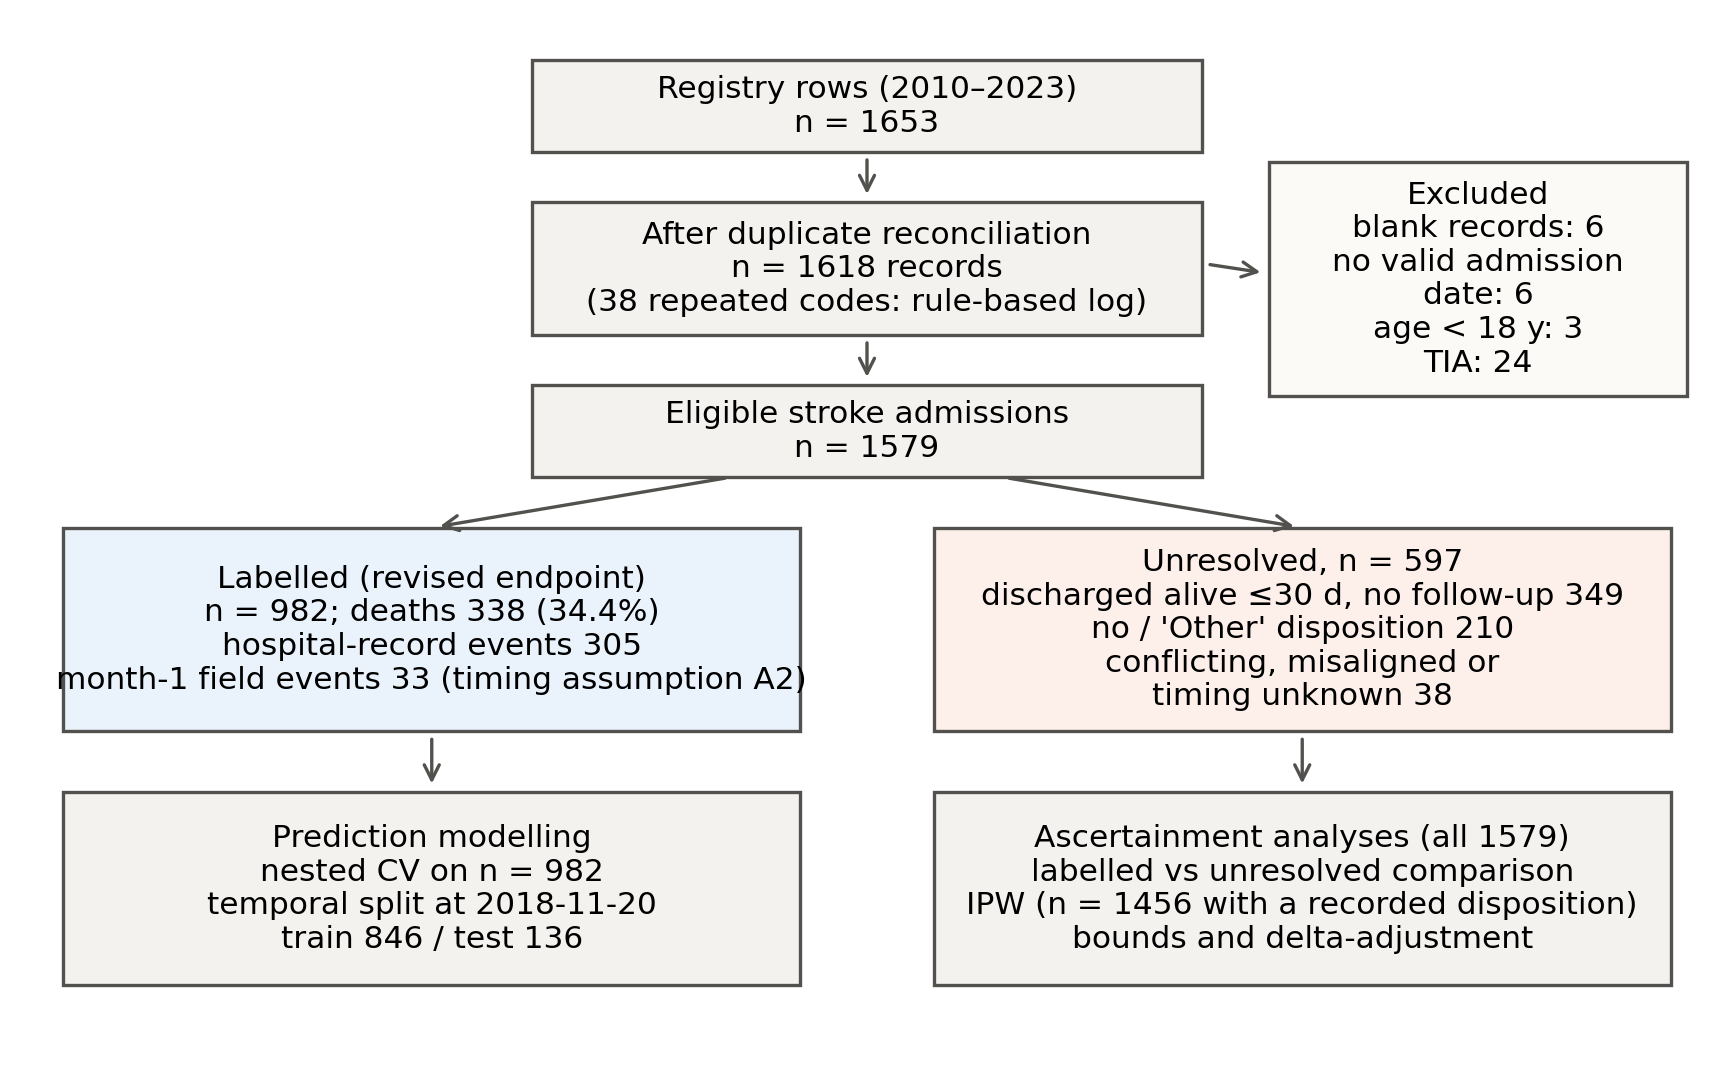
\includegraphics[width=\linewidth]{figures/fig_flow.png}
\caption{Cohort flow, outcome resolution and analysis populations. A2: timing assumption for post-discharge deaths recorded in the month-1 field.}\label{fig:flow}\end{figure}

\subsection{How first-month mortality was recorded over time}
\label{sec:res-ascert}
\linelabel{L:res-timevarying}Recording practice changed during the study period (Figure~\ref{fig:ascert}, Table~\ref{tab:period}). In 2010--2012 the month-1 field recorded \IHDeathOneEarly{} in-hospital deaths as \texttt{death1} = Yes; from 2015 it did so for \IHDeathOneLate, and the field was completed almost only for patients discharged alive. The proportion of admissions with any month-1 status fell from about 90\% to between 3\% and 61\% per year. Among labelled patients discharged alive within 30 days, the post-discharge month-1 death proportion was \PDearlyK/\PDearlyN{} (\PDearly\%) for admissions in 2010--2014 and \PDlateK/\PDlateN{} (\PDlate\%) thereafter. This suggests that post-discharge deaths were rarely captured after 2014, although a real change cannot be excluded from the data alone. Later contacts (month 3, 6 or 9) were recorded for 87\% of admissions in 2010--2012 and for 16\% or fewer from 2017; they contributed \NNfour{} survival labels. The hospital record also became less complete: disposition was missing for \DispMissTwenty{} of \AdmTwenty{} admissions in 2020, and ``Other'' became the most frequent disposition in 2021--2023 (\OtherLate{} of \AdmLate).

\begin{figure}[htbp]\centering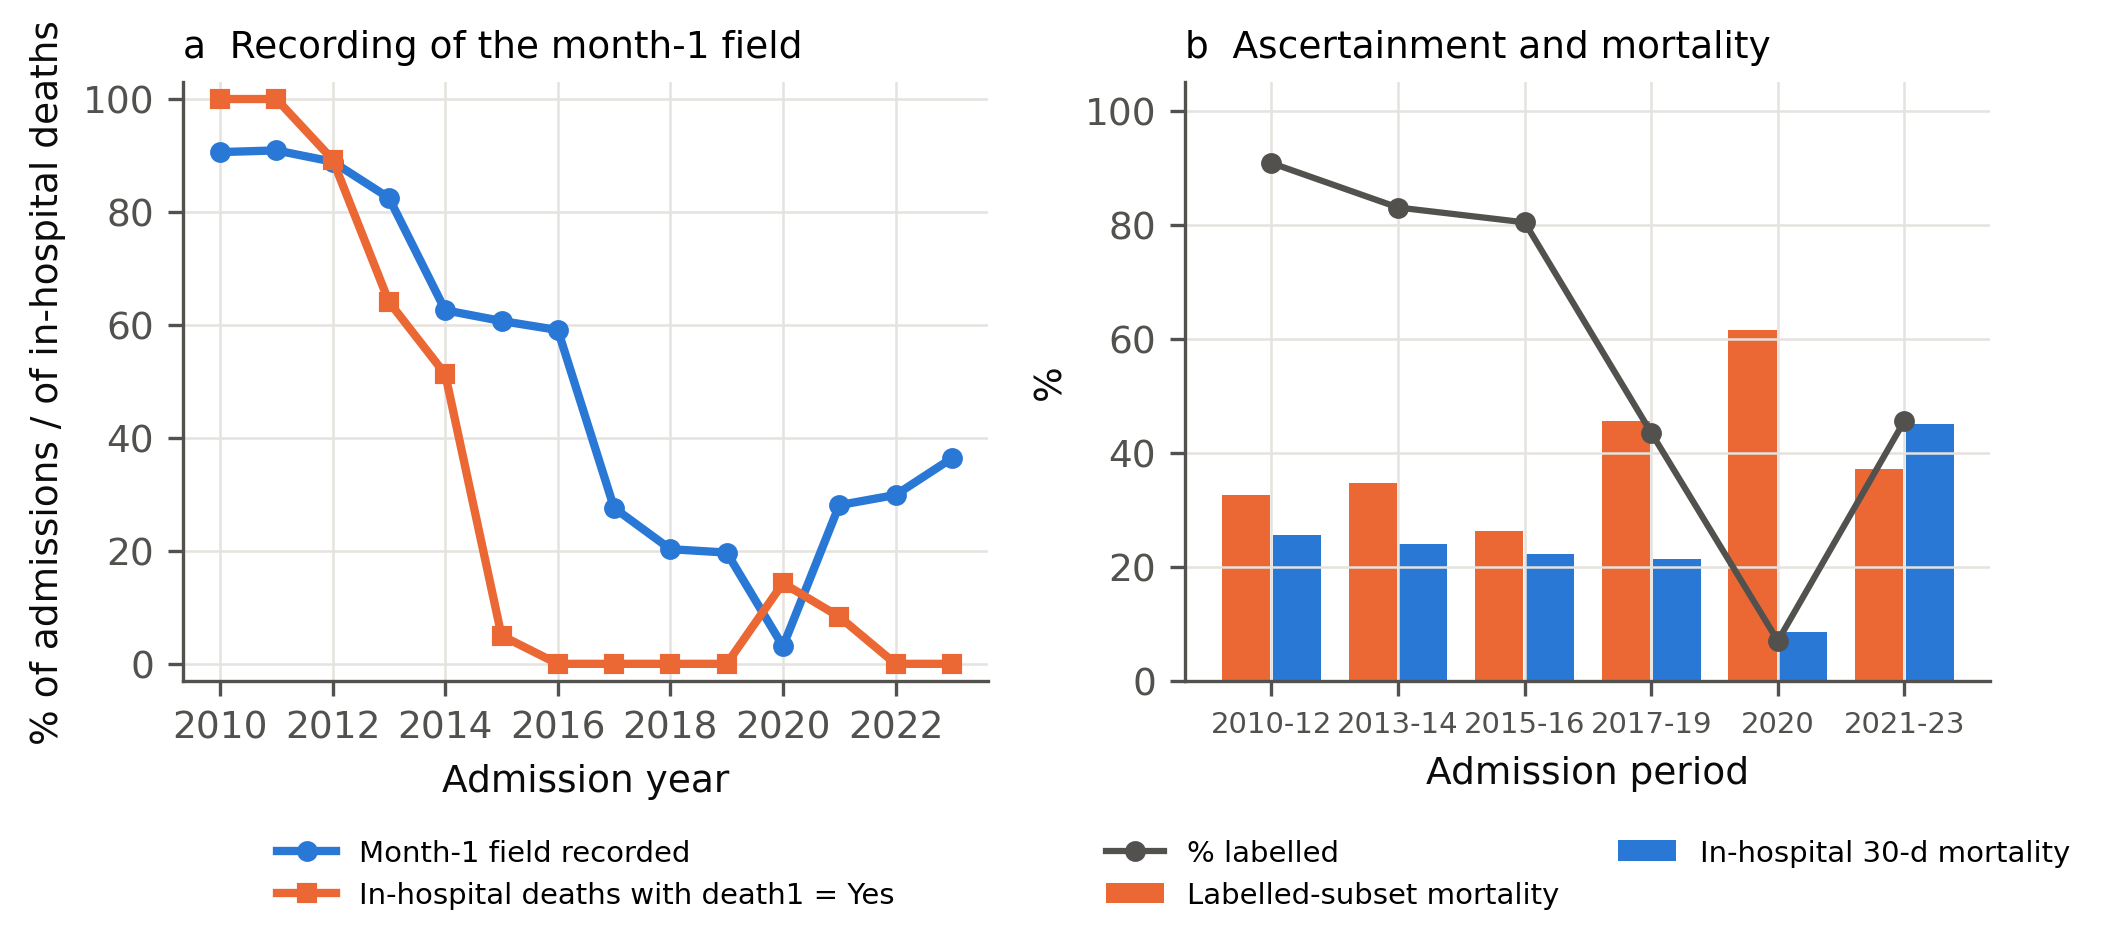
\includegraphics[width=\linewidth]{figures/fig_ascertainment.png}
\caption{Changes in outcome recording. (a) Proportion of admissions with a recorded month-1 status, and proportion of in-hospital deaths also recorded as \texttt{death1} = Yes, by admission year. (b) Proportion of eligible admissions labelled, mortality in labelled patients, and in-hospital 30-day mortality among patients with a recorded death, home or transfer disposition, by period. In 2020 most dispositions are missing, and in 2021--2023 the undocumented ``Other'' disposition is excluded from the in-hospital denominator, so those two in-hospital values are not comparable with earlier periods.}\label{fig:ascert}\end{figure}

\subsection{Label provenance and cohort-wide mortality}
\label{sec:res-mort}
\linelabel{L:res-mort}Under the revised endpoint, \Nlab{} of \Nelig{} eligible patients (62\%) were labelled, with \Ndeaths{} deaths: \NEone{} were in-hospital deaths within 30 days and \NEtwo{} were post-discharge deaths whose timing relies on assumption A2 (Table~\ref{tab:recon}). Mortality among labelled patients was \Mortlab\% (95\% CI \MortlabLo--\MortlabHi). This figure is not an estimate of registry-wide mortality. In-hospital deaths are almost always labelled, whereas survivors are labelled only when follow-up was recorded; labelled-subset mortality therefore rose to 46\% in 2017--2019 and 62\% in 2020 as the proportion labelled fell to 44\% and 7\% (Table~\ref{tab:period}). Without assumptions, cohort-wide 30-day mortality lies between \BoundLo\% and \BoundHi\% (Table~\ref{tab:reconbounds}). In-hospital 30-day mortality among patients with a known disposition was \Mortinhosp\% (95\% CI \MortinhospLo--\MortinhospHi), a lower bound for all-cause 30-day mortality in that population. The IPW estimate was \Mortipw\% (95\% CI \MortipwLo--\MortipwHi; \IPWntrunc{} weights truncated at \IPWcap; effective sample size \IPWess). Pattern-mixture estimates were \DeltaMARper\% and \DeltaMARearly\% at $\delta=1$ and ranged from \DeltaMin\% to \DeltaMax\% for $\delta$ between 0.25 and 8 (Figure~\ref{fig:delta}, Table~\ref{tab:delta}). Reproducing the labelled-subset value of \Mortlab\% would require unresolved patients to have two to four times (2010--2014 reference) or slightly more than four times (period-specific reference) the odds of death of comparable resolved patients. Under the strict endpoint, \NstrictLab{} patients were labelled with \NstrictDeaths{} deaths (\Mortstrict\%).

\begin{table}[htbp]\centering\small
\caption{Estimates of 30-day mortality among all eligible patients ($n=1{,}579$). Only the bounds are assumption-free; no single value is identified by the data.}\label{tab:reconbounds}
\begin{tabular}{>{\raggedright\arraybackslash}p{5.0cm}>{\raggedright\arraybackslash}p{2.9cm}>{\raggedright\arraybackslash}p{5.4cm}}
\toprule
Estimator & Mortality, \% (95\% CI) & Population / assumption \\
\midrule
Labelled-subset proportion & 34.4 (31.5--37.4) & Labelled patients only; selectively ascertained \\
All unresolved survived (lower bound) & 21.4 & Logical bound \\
All unresolved died (upper bound) & 59.2 & Logical bound \\
In-hospital death within 30 days & 23.6 (21.4--26.0) & Known disposition, $n=1{,}292$; excludes post-discharge deaths \\
Inverse-probability-of-observation weighted & 27.5 (25.0--30.1) & MAR given admission data, period and disposition; $n=1{,}456$ \\
Pattern-mixture, $\delta=1$ (2010--14 post-discharge risk) & 30.7 & MAR-type reference \\
Pattern-mixture, $\delta=1$ (period-specific) & 29.8 & MAR within period \\
Pattern-mixture, $\delta$ from 0.25 to 8 & 26.6--41.7 & MNAR sensitivity range \\
\bottomrule
\end{tabular}
\end{table}


\begin{figure}[htbp]\centering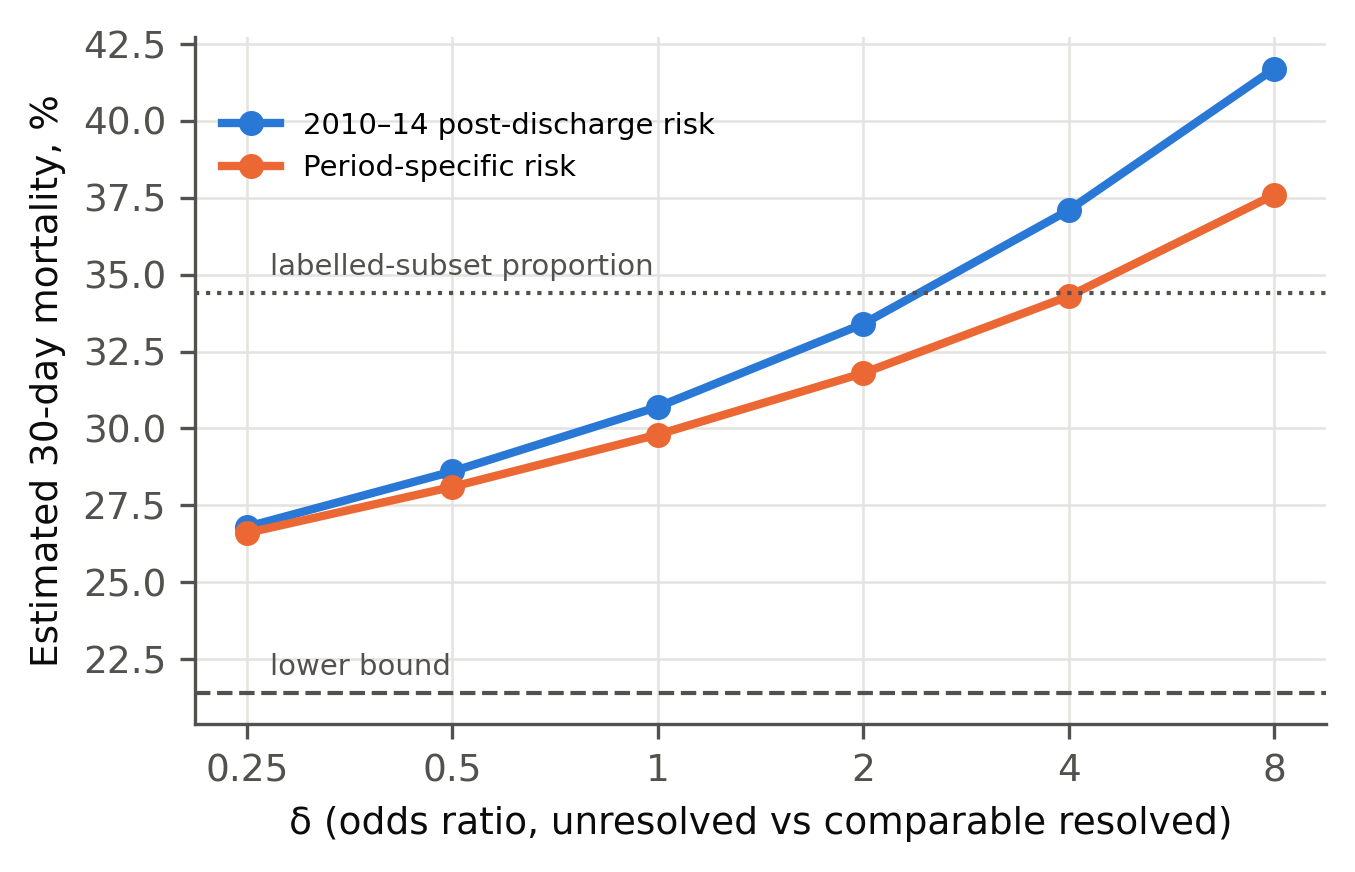
\includegraphics[width=.62\linewidth]{figures/fig_delta.png}
\caption{Delta-adjustment (pattern-mixture) sensitivity analysis of 30-day mortality among all eligible patients. $\delta$ multiplies the odds of death of unresolved patients relative to comparable resolved patients; $\delta=1$ is a missing-at-random assumption.}\label{fig:delta}\end{figure}

\subsection{Labelled versus unresolved patients}
\label{sec:res-selbias}
\linelabel{L:res-selbias}Compared with unresolved patients, labelled patients had higher NIHSS (median 10 versus 7) and admission Rankin scores (4 versus 3), lower GCS, more haemorrhagic strokes (41.6\% versus 32.4\%) and less missing NIHSS (41\% versus 58\%). Age and sex were similar (Table~\ref{tab:selbias}). The largest differences were in admission period (unresolved patients were concentrated in 2017--2023) and disposition: almost all in-hospital deaths were labelled, and 20\% of unresolved patients had no recorded disposition. Unresolved patients were therefore mostly milder patients discharged alive, or patients with undocumented dispositions, in the later years; the labelled cohort over-represents deaths relative to the registry.

\begin{table}[htbp]\centering\scriptsize
\caption{Labelled versus unresolved eligible patients (labelled $n=982$; unresolved $n=597$). Continuous variables: median [IQR] (number with a recorded value); SMD, standardised mean difference.}\label{tab:selbias}
\begin{tabular}{>{\raggedright\arraybackslash}p{3.6cm}>{\raggedright\arraybackslash}p{3.9cm}>{\raggedright\arraybackslash}p{3.9cm}r}
\toprule
Characteristic & Labelled & Unresolved & SMD \\
\midrule
Age, y & 59.0 [51.0-69.0] (n=980) & 61.0 [52.0-71.0] (n=593) & -0.13 \\
NIHSS & 10.0 [5.0-16.0] (n=576) & 7.0 [4.0-12.0] (n=249) & 0.48 \\
Glasgow Coma Scale & 14.0 [10.0-15.0] (n=947) & 15.0 [12.0-15.0] (n=470) & -0.30 \\
Modified Rankin (admission) & 4.0 [2.2-4.0] (n=514) & 3.0 [1.0-3.0] (n=252) & 0.69 \\
Systolic BP, mmHg & 165.0 [141.0-189.0] (n=968) & 160.0 [137.2-180.0] (n=454) & 0.15 \\
Creatinine, mg/dL & 1.1 [0.9-1.4] (n=808) & 1.1 [0.9-1.5] (n=426) & -0.03 \\
CRP, mg/L & 11.0 [4.0-48.0] (n=552) & 9.8 [3.4-43.5] (n=304) & 0.03 \\
Length of stay, d & 6.0 [3.0-10.0] (n=979) & 6.0 [4.0-10.0] (n=491) & -0.02 \\
Male sex & 557/982 (56.7\%) & 336/596 (56.4\%) & 0.01 \\
Haemorrhagic stroke & 407/979 (41.6\%) & 163/503 (32.4\%) & 0.19 \\
Hypertension & 683/977 (69.9\%) & 347/497 (69.8\%) & 0.00 \\
Diabetes & 207/975 (21.2\%) & 105/501 (21.0\%) & 0.01 \\
Atrial fibrillation & 41/943 (4.3\%) & 24/486 (4.9\%) & -0.03 \\
Prior stroke & 144/966 (14.9\%) & 90/494 (18.2\%) & -0.09 \\
NIHSS missing & 406/982 (41.3\%) & 348/597 (58.3\%) & -0.34 \\
mRS missing & 468/982 (47.7\%) & 345/597 (57.8\%) & -0.20 \\
CRP missing & 430/982 (43.8\%) & 293/597 (49.1\%) & -0.11 \\
Admitted 2010-12 & 295 (30.0\%) & 30 (5.0\%) & 0.70 \\
Admitted 2013-14 & 225 (22.9\%) & 46 (7.7\%) & 0.43 \\
Admitted 2015-16 & 213 (21.7\%) & 52 (8.7\%) & 0.37 \\
Admitted 2017-19 & 147 (15.0\%) & 191 (32.0\%) & -0.41 \\
Admitted 2020 & 13 (1.3\%) & 172 (28.8\%) & -0.83 \\
Admitted 2021-23 & 89 (9.1\%) & 106 (17.8\%) & -0.26 \\
Disposition: death & 307 (31.3\%) & 19 (3.2\%) &  \\
Disposition: home & 595 (60.6\%) & 354 (59.3\%) &  \\
Disposition: transfer & 20 (2.0\%) & 13 (2.2\%) &  \\
Disposition: other & 57 (5.8\%) & 91 (15.2\%) &  \\
Disposition: missing & 3 (0.3\%) & 119 (19.9\%) &  \\
\bottomrule
\end{tabular}
\end{table}


\subsection{Baseline characteristics}
Admission characteristics by outcome among labelled patients are given in Table~\ref{tab:baseline}. Patients who died had higher NIHSS, lower GCS, higher admission Rankin scores, higher blood pressure, heart and respiratory rates, and more often had haemorrhagic stroke.

\begin{table}[htbp]\centering\scriptsize
\caption{Admission characteristics of labelled patients by outcome (survived $n=644$; died $n=338$). Median [IQR] or $n$ (\%); missing \% refers to the labelled cohort; Mann--Whitney or $\chi^2$ test.}\label{tab:baseline}
\begin{tabular}{>{\raggedright\arraybackslash}p{4.2cm}>{\raggedright\arraybackslash}p{2.8cm}>{\raggedright\arraybackslash}p{2.8cm}rr}
\toprule
Characteristic & Survived & Died & Missing \% & $p$ \\
\midrule
Age, y & 58.0 [51.0-68.5] & 60.0 [52.0-69.0] & 0.2 & 0.152 \\
NIHSS & 8.0 [4.0-12.0] & 16.5 [12.0-22.0] & 41.3 & $<$0.001 \\
Glasgow Coma Scale & 15.0 [13.0-15.0] & 9.0 [7.0-13.0] & 3.6 & $<$0.001 \\
Modified Rankin (admission) & 3.0 [2.0-4.0] & 4.0 [4.0-5.0] & 47.7 & $<$0.001 \\
Systolic BP, mmHg & 160.0 [140.0-182.0] & 173.0 [144.2-198.5] & 1.4 & $<$0.001 \\
Heart rate, /min & 81.0 [72.0-93.0] & 88.0 [74.0-105.8] & 3.5 & $<$0.001 \\
Respiratory rate, /min & 20.0 [18.0-24.0] & 24.0 [20.0-28.0] & 36.9 & $<$0.001 \\
Temperature, $^\circ$C & 37.0 [36.8-37.5] & 37.2 [36.9-38.0] & 5.1 & $<$0.001 \\
Capillary glucose, g/L & 1.2 [1.0-1.6] & 1.4 [1.1-1.8] & 26.1 & $<$0.001 \\
Creatinine, mg/dL & 1.1 [0.9-1.4] & 1.2 [0.9-1.8] & 17.7 & $<$0.001 \\
Urea, g/L & 0.3 [0.2-0.4] & 0.4 [0.3-0.7] & 24.2 & $<$0.001 \\
White-cell count, $\times10^3/\mu$L & 6.4 [5.2-8.2] & 8.4 [5.9-11.9] & 8.2 & $<$0.001 \\
CRP, mg/L & 7.0 [4.0-24.0] & 28.4 [6.0-99.8] & 43.8 & $<$0.001 \\
Haemoglobin, g/dL & 12.9 [11.5-14.1] & 13.1 [11.6-14.6] & 7.0 & 0.151 \\
Male sex & 367 (57.0) & 190 (56.2) & 0.0 & 0.869 \\
Haemorrhagic stroke & 203 (31.6) & 204 (60.7) & 0.3 & $<$0.001 \\
Hypertension & 448 (69.6) & 235 (70.6) & 0.5 & 0.802 \\
Diabetes & 137 (21.3) & 70 (21.0) & 0.7 & 0.974 \\
Atrial fibrillation & 19 (3.1) & 22 (6.7) & 4.0 & 0.015 \\
Prior stroke & 91 (14.4) & 53 (15.9) & 1.6 & 0.587 \\
\bottomrule
\end{tabular}
\end{table}


\subsection{Discrimination}
\label{sec:res-disc}
\linelabel{L:res-disc}In nested cross-validation ($n=\Nlab$; \Ndeaths{} deaths; \EPV{} events per candidate predictor), the primary model achieved a pooled out-of-fold AUROC of \NestLR{} (95\% CI \NestLRLo--\NestLRHi; fold mean \NestLRFold{} $\pm$ \NestLRFoldSD) and an AUPRC of \NestLRAP{} (Table~\ref{tab:nestedcv}, Figure~\ref{fig:roc}a). The random forest performed similarly (\NestRF), and histogram gradient boosting (\NestHGB) and XGBoost (\NestXGB) were slightly higher (XGBoost minus primary \PairXGBDiff, 95\% CI \PairXGBLo{} to \PairXGBHi).

\begin{table}[htbp]\centering\scriptsize
\caption{Nested cross-validation (5 outer folds $\times$ 5 repeats; inner 3-fold tuning) on the labelled cohort ($n=982$, 338 deaths). Pooled AUROC uses out-of-fold predictions averaged over repeats (DeLong 95\% CI); fold AUROC is mean $\pm$ SD over the 25 outer test folds. Calibration slope, intercept and Brier score are means over the 5 repeats of pooled out-of-fold predictions.}\label{tab:nestedcv}
\begin{tabular}{>{\raggedright\arraybackslash}p{3.6cm}>{\raggedright\arraybackslash}p{2.7cm}>{\raggedright\arraybackslash}p{2.1cm}rrrr}
\toprule
Model & Pooled AUROC (95\% CI) & Fold AUROC & AUPRC & Slope & Intercept & Brier \\
\midrule
L2 logistic regression (primary) & 0.863 (0.839--0.886) & 0.862 $\pm$ 0.020 & 0.771 & 1.14 & -0.01 & 0.143 \\
Clinical-reference model & 0.839 (0.813--0.865) & 0.839 $\pm$ 0.022 & 0.759 & 0.97 & 0.00 & 0.150 \\
Random forest & 0.862 (0.837--0.887) & 0.861 $\pm$ 0.023 & 0.788 & 1.19 & -0.01 & 0.139 \\
Histogram gradient boosting & 0.877 (0.854--0.900) & 0.872 $\pm$ 0.025 & 0.813 & 0.99 & 0.02 & 0.132 \\
XGBoost & 0.878 (0.855--0.901) & 0.876 $\pm$ 0.025 & 0.817 & 0.95 & 0.04 & 0.130 \\
\bottomrule
\end{tabular}
\end{table}


\begin{figure}[htbp]\centering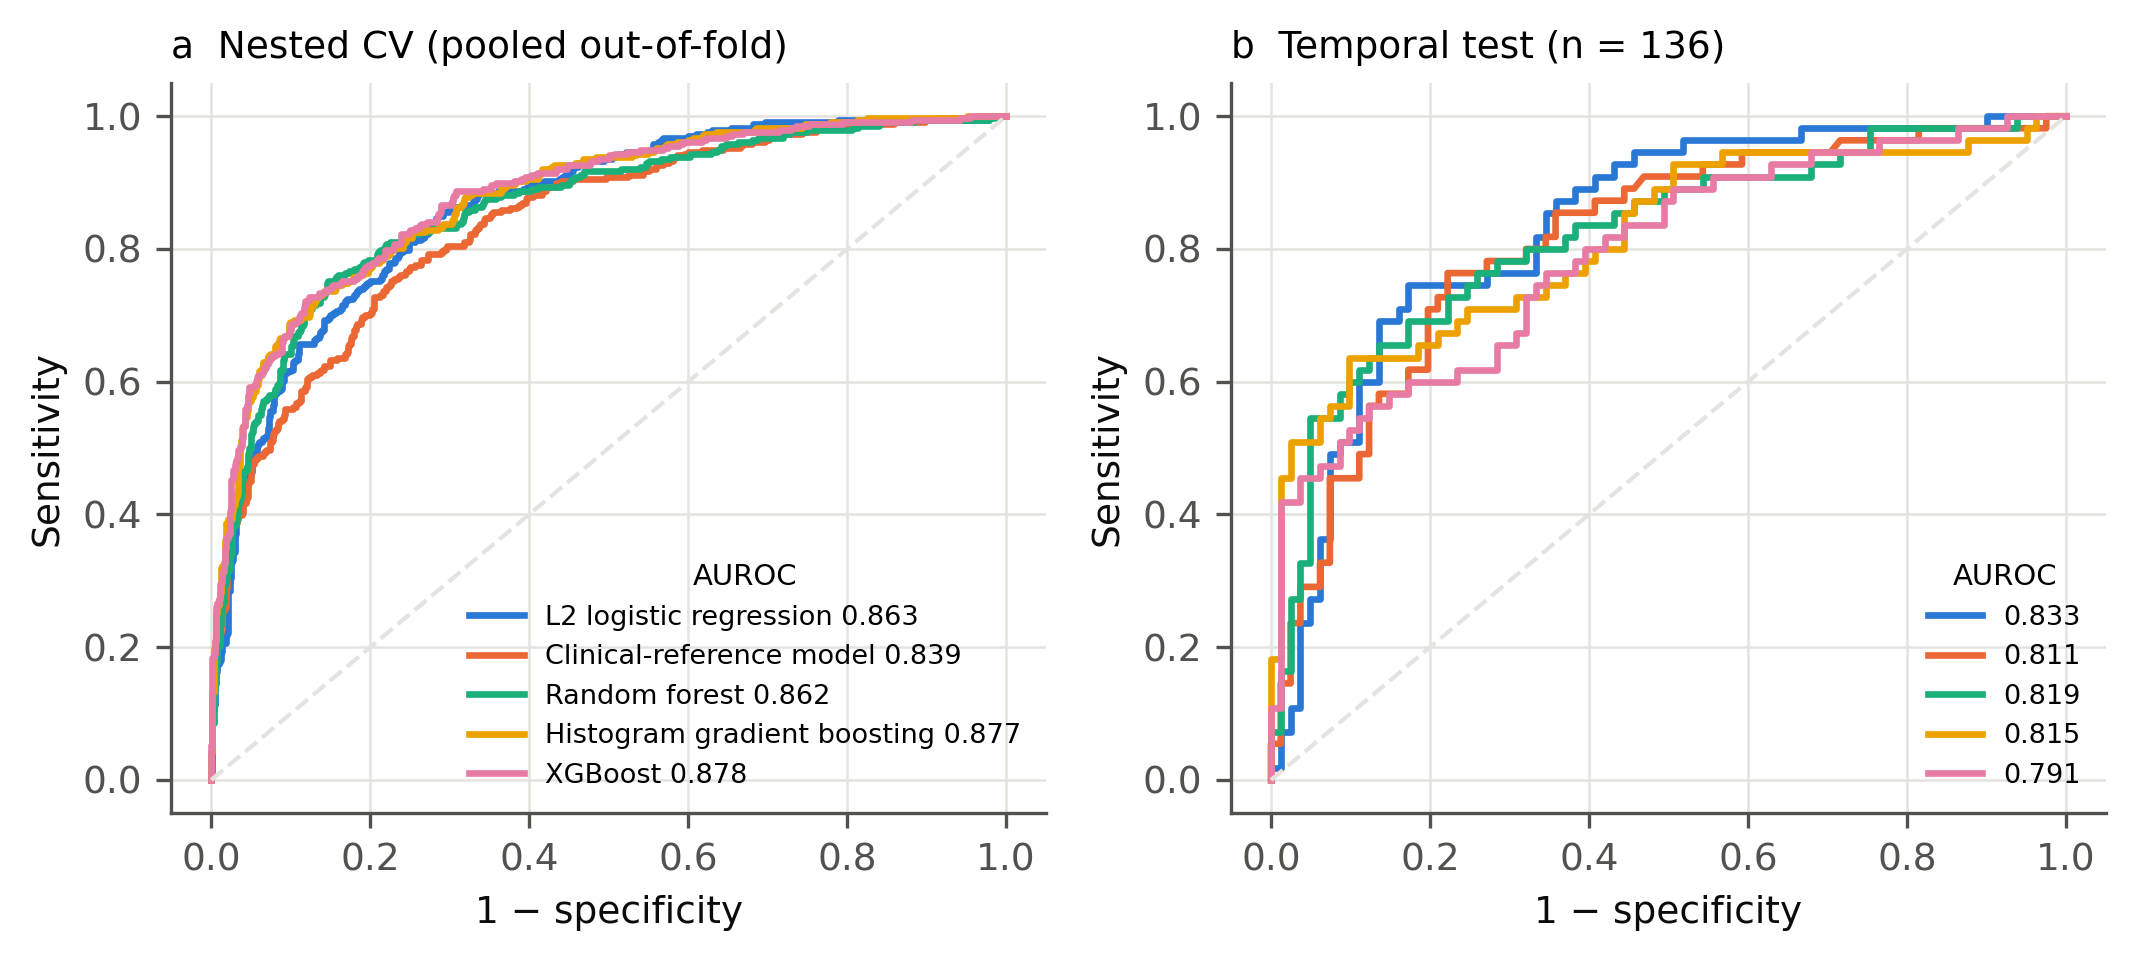
\includegraphics[width=\linewidth]{figures/fig_roc.png}
\caption{ROC curves. (a) Pooled out-of-fold predictions from nested cross-validation (averaged over five repeats). (b) Temporal test set (admissions from \TCut).}\label{fig:roc}\end{figure}

\subsection{Comparison with the clinical-reference model}
\label{sec:res-paired}
\linelabel{L:res-paired}The clinical-reference model achieved \NestCR{} (95\% CI \NestCRLo--\NestCRHi). On the same patients the paired AUROC difference (primary minus reference) was \PairNestDiff{} (95\% CI \PairNestLo{} to \PairNestHi; DeLong $p$ \PairNestP), and the primary model was higher in \FoldLRBetter{} of \NFolds{} outer folds (mean fold difference \FoldDiffMean{} $\pm$ \FoldDiffSD). Because the pooled out-of-fold predictions come from different training sets, this DeLong interval is approximate. On the temporal test set the difference was \TPairDiff{} (95\% CI \TPairLo{} to \TPairHi; $p=\TPairP$; Table~\ref{tab:paireddelong}). The data are compatible with no difference and with a gain of up to 0.07; they establish neither equivalence nor superiority.

\begin{table}[htbp]\centering\small
\caption{Paired comparison of the primary model with the clinical-reference model (DeLong). A non-significant difference is not evidence of equivalence; no equivalence margin was pre-specified.}\label{tab:paireddelong}
\begin{tabular}{>{\raggedright\arraybackslash}p{4.0cm}rr>{\raggedright\arraybackslash}p{3.4cm}r}
\toprule
Setting & AUROC primary & AUROC reference & Difference (95\% CI) & $p$ \\
\midrule
Nested CV (pooled out-of-fold) & 0.863 & 0.839 & 0.024 (0.010 to 0.038) & $<$0.001 \\
Temporal test ($n=136$) & 0.833 & 0.811 & 0.022 (-0.027 to 0.070) & 0.38 \\
\bottomrule
\end{tabular}
\end{table}


\subsection{Temporal validation}
\label{sec:res-temporal}
\linelabel{L:res-temporal}Models developed on \TNtr{} labelled admissions before \TCut{} (\TEtr{} deaths) were tested on \TNte{} later admissions (\TEte{} deaths, \TPrev\%). The primary model's AUROC was \TLR{} (95\% CI \TLRLo--\TLRHi), the clinical reference \TCR{}, and the tree ensembles \TEnsLo--\TEnsHi{} (Table~\ref{tab:temporal}, Figure~\ref{fig:roc}b). The strict endpoint gave \TStLR{} (\TStN{} patients, \TStE{} deaths). Under the observed-only endpoint the test set contained only \TObE{} deaths among \TObN{} patients, because in-hospital deaths were no longer written into \texttt{death1}. Its AUROC (\TObLR, 95\% CI \TObLRLo--\TObLRHi) is too imprecise to interpret, and with a common cut-off the collapse reported in the earlier version did not recur. The later period differed from the earlier one in case mix and missingness (a model predicting the period from the predictors had a cross-validated AUROC of \TMember), in the proportion labelled and in the share of labels derived from hospital records (Table~\ref{tab:tempshift}). These shifts coincide with the change in outcome recording, so the temporal results cannot separate case-mix shift from recording change.

\begin{table}[htbp]\centering\scriptsize
\caption{Temporal validation: training on admissions before 2018-11-20 and testing on later admissions (cut-off = 70th percentile of admission dates among all eligible patients; identical for every endpoint). $n$/deaths shown for training and test sets.}\label{tab:temporal}
\begin{tabular}{>{\raggedright\arraybackslash}p{2.6cm}>{\raggedright\arraybackslash}p{2.8cm}rr>{\raggedright\arraybackslash}p{2.6cm}rr}
\toprule
Endpoint & Model & Train $n$/deaths & Test $n$/deaths & AUROC (95\% CI) & Slope & Intercept \\
\midrule
Revised primary endpoint & L2 logistic regression & 846/283 & 136/55 & 0.833 (0.764--0.902) & 1.23 & 0.72 \\
 & Clinical-reference model & 846/283 & 136/55 & 0.811 (0.737--0.886) & 1.00 & 0.85 \\
 & Random forest & 846/283 & 136/55 & 0.819 (0.744--0.893) & 1.09 & 0.71 \\
 & Histogram gradient boosting & 846/283 & 136/55 & 0.815 (0.738--0.891) & 0.89 & 0.77 \\
 & XGBoost & 846/283 & 136/55 & 0.791 (0.713--0.869) & 0.49 & 1.18 \\
Strict admission-timed endpoint & L2 logistic regression & 815/252 & 134/53 & 0.833 (0.764--0.903) & 1.17 & 0.85 \\
 & Clinical-reference model & 815/252 & 134/53 & 0.815 (0.741--0.888) & 0.94 & 0.96 \\
Observed-only \texttt{death1} & L2 logistic regression & 701/156 & 83/4 & 0.867 (0.758--0.976) & 1.02 & -1.20 \\
 & Clinical-reference model & 701/156 & 83/4 & 0.858 (0.743--0.972) & 0.77 & -1.06 \\
\bottomrule
\end{tabular}
\end{table}


\subsection{Calibration}
\label{sec:res-calib}
\linelabel{L:res-calib}Out-of-fold predictions of the primary model had a calibration intercept of \NestLRInt{} and slope of \NestLRSlope{} (Brier \NestLRBrier; Table~\ref{tab:recal}, Figure~\ref{fig:cal}a); a slope above 1 indicates that the penalised model's predictions were slightly too conservative. In-fold Platt scaling gave a slope of \RecPlattSlope{} and isotonic regression \RecIsoSlope{}, with Brier scores of \RecPlattBrier{} and \RecIsoBrier; neither was adopted. On the temporal test set the model under-predicted (intercept \TLRInt, slope \TLRSlope; Figure~\ref{fig:cal}b), as expected when survivors in the later period are under-ascertained; with IPW weights the intercept was \TLRipwInt{} and the slope \TLRipwSlope. With IPW weights on the out-of-fold predictions the mean predicted risk (\NestLRipwMeanPred\%) exceeded the weighted observed proportion (\NestLRipwObs\%; intercept \NestLRipwInt). Absolute risks from this model therefore reflect the ascertainment of the development data, not the registry population.

\begin{figure}[htbp]\centering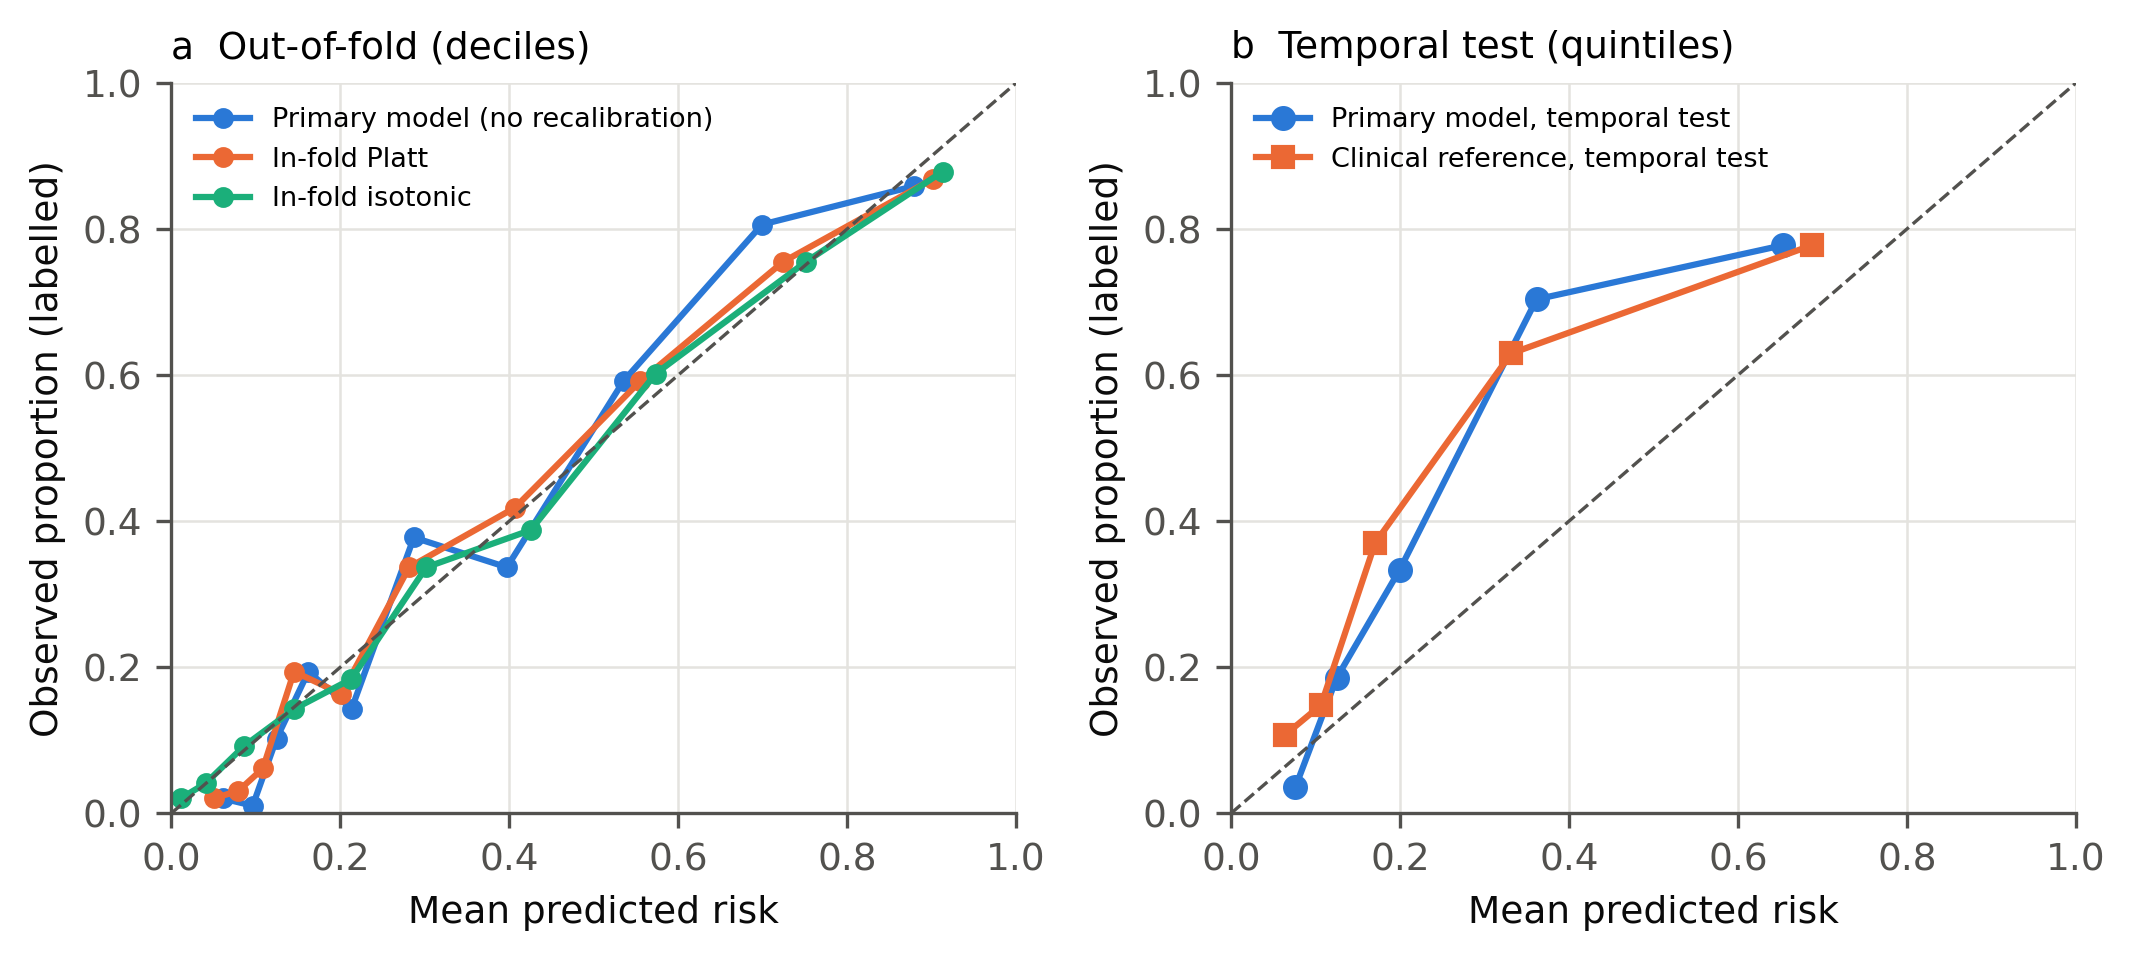
\includegraphics[width=\linewidth]{figures/fig_calibration.png}
\caption{Calibration of the primary model. (a) Out-of-fold predictions without recalibration and with in-fold Platt or isotonic recalibration (deciles). (b) Temporal test set (quintiles). Observed proportions refer to labelled patients.}\label{fig:cal}\end{figure}

\subsection{Risk tiers and decision curves}
\label{sec:res-tiers}
\linelabel{L:res-tiers}At the pre-specified cut-points, the low-risk tier contained \TierOLowPct\% of patients with an observed mortality of \TierOLowMort\% on out-of-fold predictions, and the high-risk tier \TierOHighPct\% of patients with \TierOHighMort\% mortality and \TierOHighCap\% of deaths (Table~\ref{tab:tiers}, Figure~\ref{fig:tiers}). On the temporal test set the low tier contained \TierTLowN{} patients (\TierTLowPct\%; mortality \TierTLowMort\%), and the high tier captured \TierTHighCap\% of deaths. The earlier finding that no low-risk tier emerged resulted from tuning thresholds on a small validation split and did not recur. As an illustration of follow-up effort, the high tier contained \TierOHighPPD{} patients per death and the low tier \TierOLowPPD{} patients per death on out-of-fold predictions (Table~\ref{tab:tiers}). These figures refer to the labelled, selectively ascertained cohort and cannot be read as patient-level risks or as resource consequences in the registry population. Decision curves showed higher net benefit for the primary model than for treating all patients over most of the 5--50\% threshold range, both unweighted and IPW-weighted, but the curves depend on the distorted prevalence and do not demonstrate clinical benefit (Figure~\ref{fig:dca}).

\begin{table}[htbp]\centering\footnotesize
\caption{Risk tiers at pre-specified absolute-risk cut-points (low $<$10\%, high $\ge$40\%). Mortality refers to the labelled, selectively ascertained cohort and is not a population risk. Patients per death: number of patients in the tier for each death it contains, an illustration of follow-up effort per death reached if follow-up were directed to that tier.}\label{tab:tiers}
\begin{tabular}{llrrrrr}
\toprule
Setting & Tier & Patients (\%) & Deaths & Mortality \% (95\% CI) & \% of deaths & Patients per death \\
\midrule
Pooled out-of-fold & Low & 158 (16.1) & 3 & 1.9 (0.6--5.4) & 0.9 & 52.7 \\
 & Moderate & 478 (48.7) & 95 & 19.9 (16.5--23.7) & 28.1 & 5.0 \\
 & High & 346 (35.2) & 240 & 69.4 (64.3--74.0) & 71.0 & 1.4 \\
Temporal test & Low & 26 (19.1) & 1 & 3.8 (0.7--18.9) & 1.8 & 26.0 \\
 & Moderate & 73 (53.7) & 26 & 35.6 (25.6--47.1) & 47.3 & 2.8 \\
 & High & 37 (27.2) & 28 & 75.7 (59.9--86.6) & 50.9 & 1.3 \\
\bottomrule
\end{tabular}
\end{table}


\begin{figure}[htbp]\centering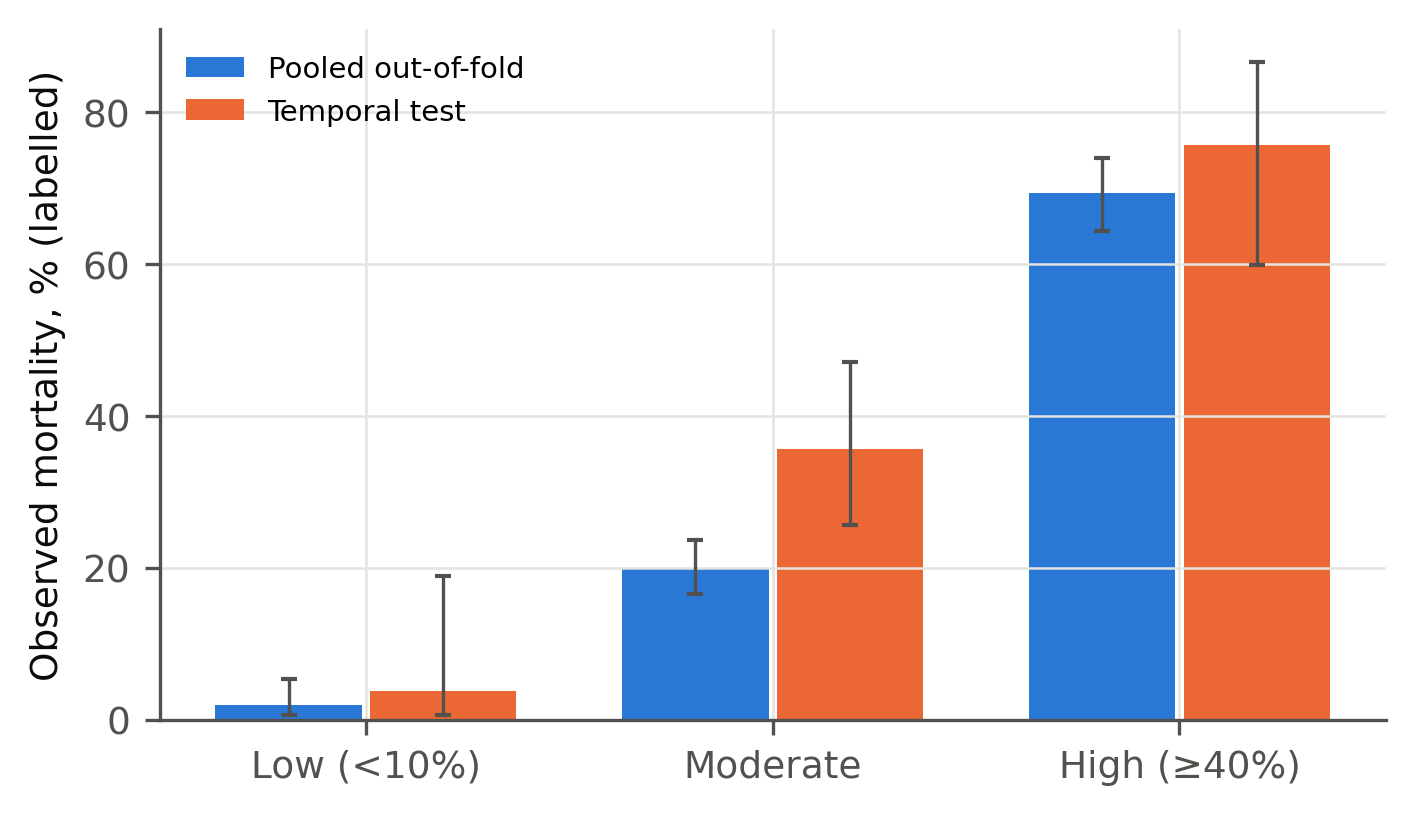
\includegraphics[width=.6\linewidth]{figures/fig_tiers.png}
\caption{Observed mortality (labelled patients) by pre-specified risk tier, with Wilson 95\% CIs.}\label{fig:tiers}\end{figure}

\begin{figure}[htbp]\centering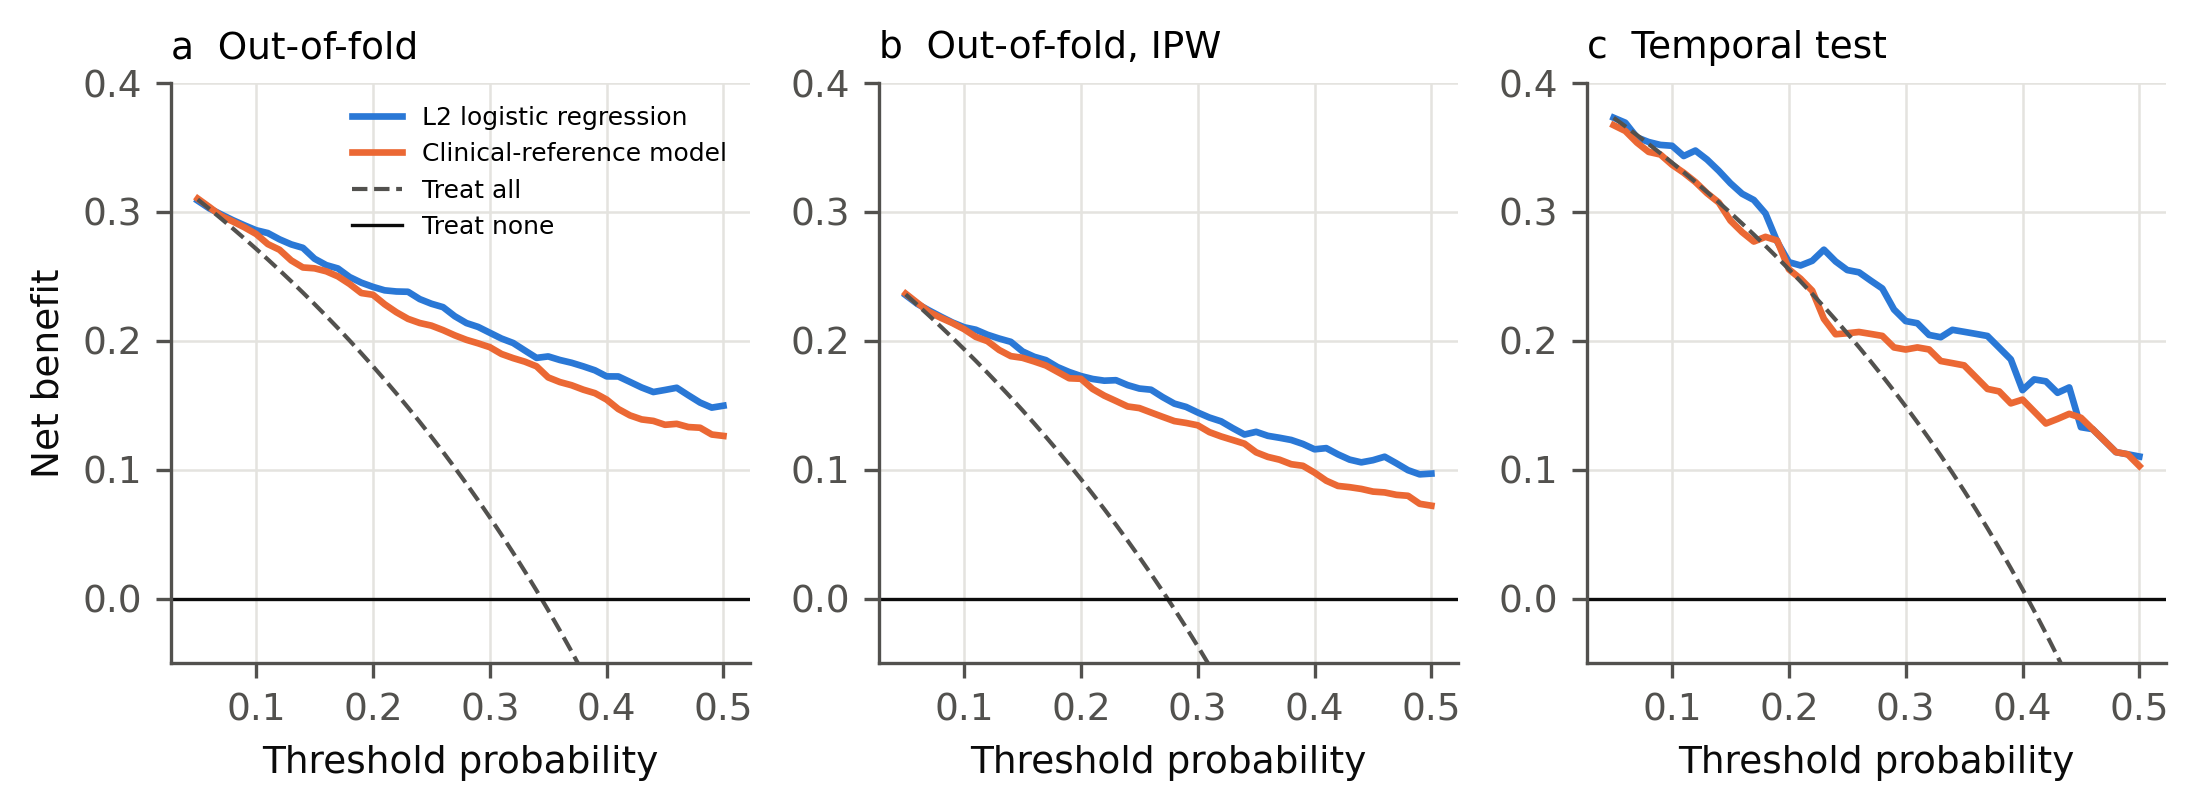
\includegraphics[width=\linewidth]{figures/fig_dca.png}
\caption{Decision curves for the primary and clinical-reference models: (a) out-of-fold, (b) out-of-fold with IPW weights, (c) temporal test set. Exploratory; net benefit depends on outcome prevalence, which is affected by selective ascertainment.}\label{fig:dca}\end{figure}

\subsection{Model interpretation}
\label{sec:res-interp}
\linelabel{L:res-interp}GCS, NIHSS and haemorrhagic subtype had the largest coefficients and SHAP values in the primary model, followed by urea, systolic blood pressure, CRP, respiratory rate and age (Table~\ref{tab:interp}, Figure~\ref{fig:shap}). GCS and NIHSS were also the two most important features for XGBoost, but the rank agreement between the two models across all \NFeat{} predictors was moderate (Spearman $\rho=\ShapRho$; feature-bootstrap interval \ShapRhoLo--\ShapRhoHi). Adding the Glasgow-to-NIHSS ratio did not improve discrimination (AUROC \SensRa{} versus \NestLR), so we no longer present it as a distinct prognostic signal.

\begin{table}[htbp]\centering\scriptsize
\caption{Final primary model ($C=0.03$): odds ratio per standard deviation (binary: per unit change after standardisation) with bootstrap 95\% CI (200 resamples), frequency of a top-5 rank across bootstrap refits, mean $|$SHAP$|$ for the primary model and XGBoost, and permutation importance (AUROC drop) on the temporal test set. Twelve largest coefficients shown; associations are not causal.}\label{tab:interp}
\begin{tabular}{>{\raggedright\arraybackslash}p{3.3cm}>{\raggedright\arraybackslash}p{2.7cm}rrrr}
\toprule
Predictor & OR per SD (95\% CI) & Top-5 freq. & $|$SHAP$|$ LR & $|$SHAP$|$ XGB & Perm. drop \\
\midrule
Glasgow Coma Scale & 0.50 (0.43--0.58) & 1.00 & 0.597 & 0.840 & 0.105 \\
NIHSS & 1.44 (1.28--1.63) & 0.95 & 0.296 & 0.344 & 0.005 \\
Haemorrhagic subtype & 1.34 (1.19--1.53) & 0.77 & 0.281 & 0.158 & 0.019 \\
Urea & 1.33 (1.15--1.61) & 0.60 & 0.163 & 0.117 & 0.017 \\
CRP & 1.26 (1.08--1.47) & 0.34 & 0.152 & 0.174 & 0.012 \\
Respiratory rate & 1.23 (1.06--1.39) & 0.22 & 0.146 & 0.184 & 0.004 \\
Systolic BP & 1.22 (1.05--1.43) & 0.22 & 0.161 & 0.167 & 0.003 \\
Smoking & 0.83 (0.72--0.96) & 0.17 & 0.121 & 0.052 & 0.002 \\
Age & 1.20 (1.07--1.36) & 0.12 & 0.144 & 0.237 & 0.004 \\
Creatinine & 1.19 (0.98--1.47) & 0.20 & 0.087 & 0.124 & 0.014 \\
Haemoglobin & 1.17 (1.03--1.35) & 0.11 & 0.118 & 0.094 & 0.000 \\
Modified Rankin (admission) & 1.15 (1.04--1.34) & 0.09 & 0.113 & 0.115 & 0.017 \\
\bottomrule
\end{tabular}
\end{table}


\begin{figure}[htbp]\centering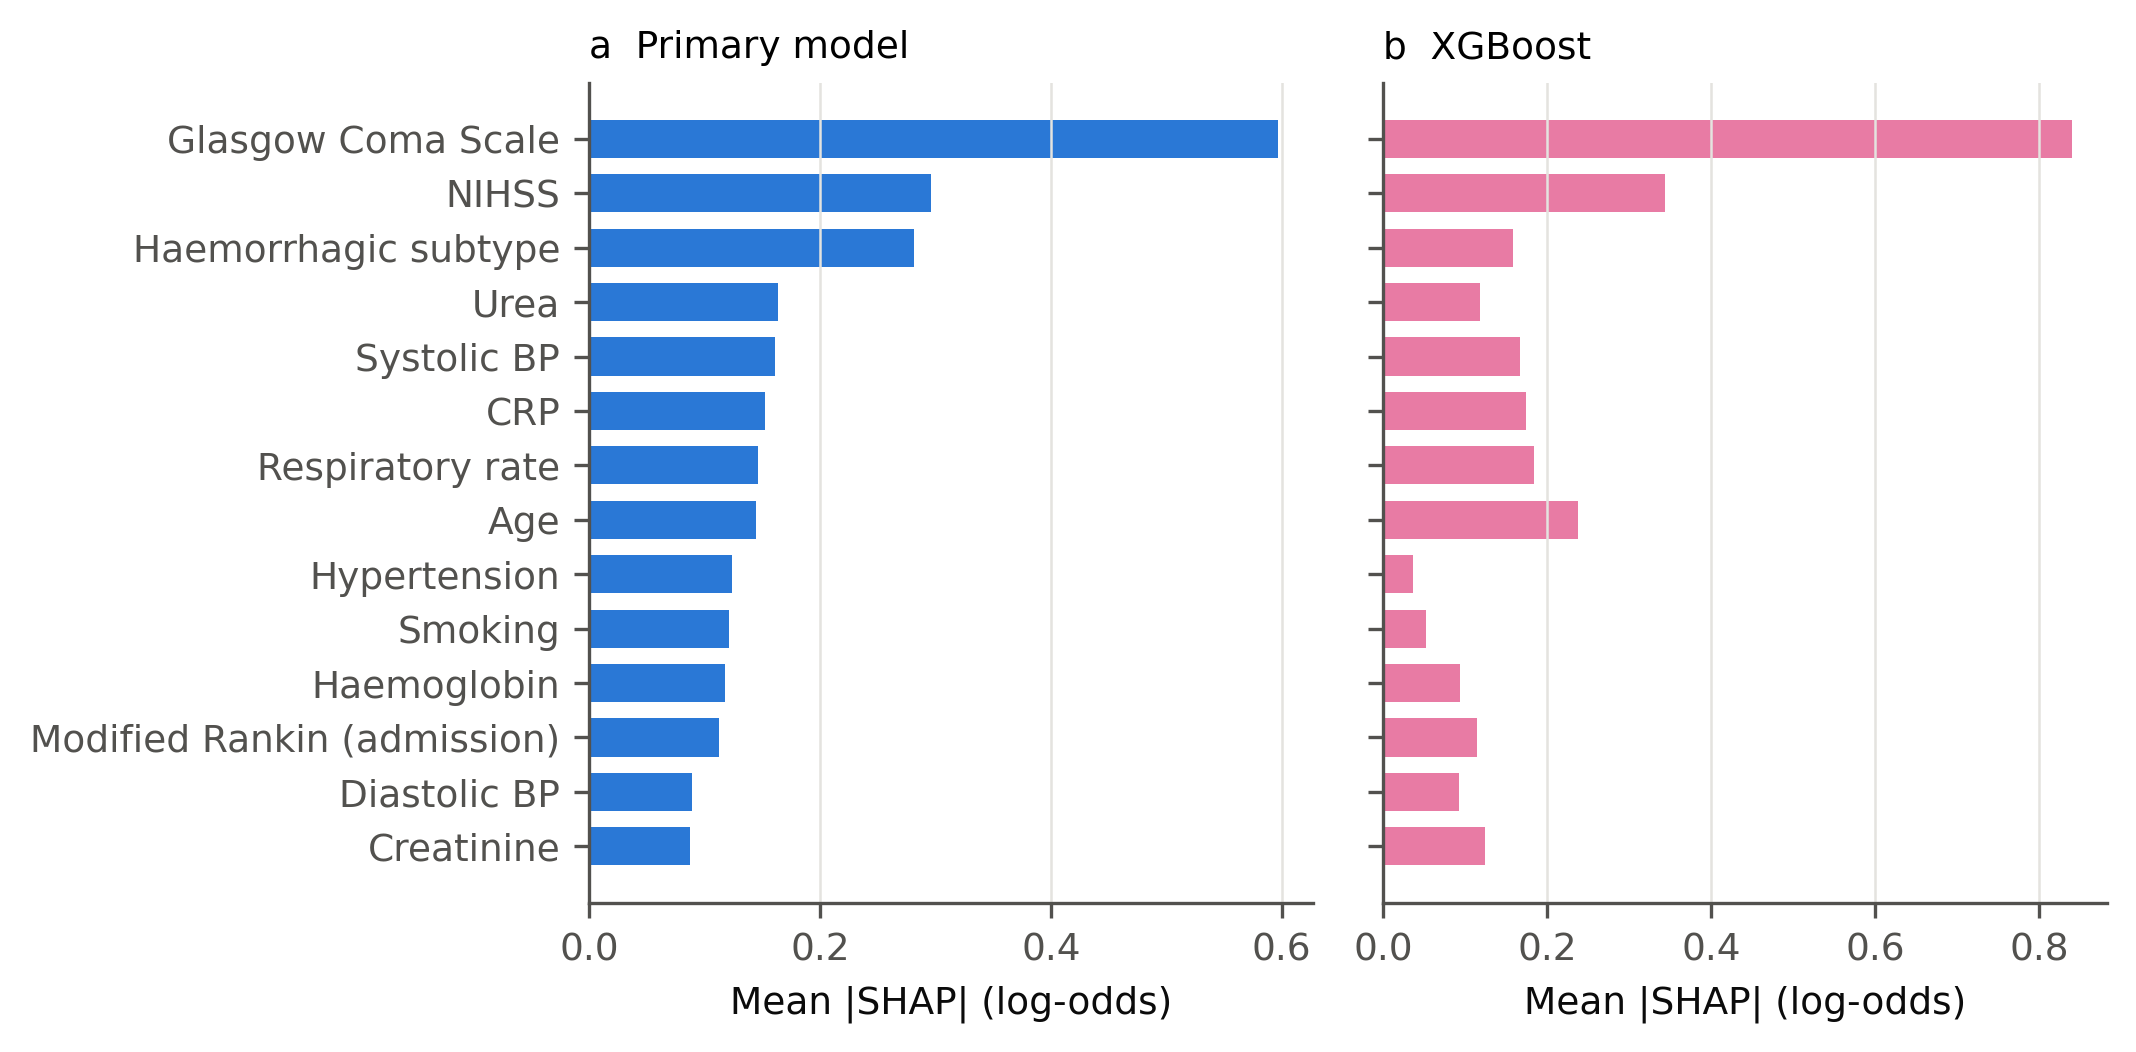
\includegraphics[width=\linewidth]{figures/fig_shap.png}
\caption{Mean absolute SHAP values (log-odds scale) for (a) the primary model and (b) XGBoost, both fitted on all labelled patients; the 14 predictors with the largest values in the primary model are shown. Importance describes model behaviour and is not causal.}\label{fig:shap}\end{figure}

\subsection{Sensitivity and subgroup analyses}
\label{sec:sensitivity}
\linelabel{L:res-sens}Discrimination was stable across endpoint definitions, duplicate rules and missing-data strategies (Table~\ref{tab:sens}). The strict endpoint gave \SensSt{} and the observed-only endpoint \SensOb; restricting to 2010--2016 gave \SensEra; removing the later-contact labels gave \SensNl; treating \texttt{death1} = No as unresolved when the onset-to-arrival delay exceeded 72 hours gave \SensOg{} ($n=\SensOgN$), and \SensOu{} when unknown delays were also excluded ($n=\SensOuN$); IPW-weighted fitting and evaluation gave \SensIw. Multiple imputation with five posterior draws gave \SensMi{} (between-draw SD of fold AUROC \MIdrawSD). Missingness indicators for NIHSS alone or for all \NhiMiss{} predictors with more than 20\% missing gave \SensNi{} and \SensMa. The model restricted to the \NlowMiss{} predictors with less than 10\% missing gave \SensLm. The complete-NIHSS subset had higher discrimination (\SensCn). Calibration slopes were further from 1 in the observed-only, 2010--2016 and complete-NIHSS analyses. Across subgroups AUROC ranged from \SGnihssMiss{} (NIHSS missing) to \SGnihssRec{} (NIHSS recorded), with overlapping intervals; the calibration intercept was \SGearlyInt{} for admissions in 2010--2016 and \SGlateInt{} for 2017--2023 (Table~\ref{tab:subgroups}).

\begin{table}[htbp]\centering\scriptsize
\caption{Sensitivity analyses (nested CV, 5 outer folds $\times$ 2 repeats). IPW row: weighted AUROC without DeLong interval. Multiple imputation: penalty fixed at $C=0.03$; between-draw SD of fold AUROC 0.010.}\label{tab:sens}
\begin{tabular}{>{\raggedright\arraybackslash}p{4.6cm}r>{\raggedright\arraybackslash}p{3.0cm}rrr}
\toprule
Analysis & $n$/deaths & AUROC primary (95\% CI) & AUROC reference & Slope & Intercept \\
\midrule
Strict admission-timed endpoint & 949/305 & 0.872 (0.848--0.895) & 0.847 & 1.20 & 0.00 \\
Observed-only \texttt{death1} & 784/160 & 0.868 (0.837--0.900) & 0.845 & 1.76 & -0.02 \\
Duplicates: keep first row & 982/340 & 0.858 (0.833--0.882) & 0.839 & 1.17 & 0.01 \\
Duplicates: exclude conflicting groups & 979/337 & 0.854 (0.829--0.878) & 0.838 & 1.22 & 0.01 \\
Admissions 2010--2016 only & 733/230 & 0.859 (0.831--0.888) & 0.840 & 1.71 & 0.00 \\
Complete NIHSS only & 576/186 & 0.885 (0.857--0.913) & 0.887 & 1.81 & 0.02 \\
Later-contact survival (N4) treated as unresolved & 962/338 & 0.859 (0.834--0.883) & -- & 1.14 & 0.01 \\
Stroke-anchored month 1: \texttt{death1} = No with onset-to-arrival delay $>$72 h unresolved & 873/338 & 0.856 (0.831--0.881) & -- & 1.22 & 0.00 \\
As above, and \texttt{death1} = No with unknown delay unresolved & 806/338 & 0.855 (0.829--0.881) & -- & 1.22 & 0.01 \\
NIHSS missingness indicator added & 982/338 & 0.866 (0.843--0.889) & -- & 1.24 & 0.00 \\
Missingness indicators for all predictors $>$20\% missing & 982/338 & 0.869 (0.845--0.892) & -- & 1.31 & 0.00 \\
Predictors $<$10\% missing only & 982/338 & 0.834 (0.808--0.861) & -- & 1.27 & 0.00 \\
Glasgow-to-NIHSS ratio added & 982/338 & 0.861 (0.837--0.885) & -- & 1.10 & -0.01 \\
Multiple imputation, $m=5$ posterior draws & 982/338 & 0.864 (0.840--0.887) & -- & 1.23 & 0.00 \\
IPW-weighted fitting and evaluation & 982/338 & 0.861 (0.837--0.885) & 0.838 & 1.23 & 0.27 \\
\bottomrule
\end{tabular}
\end{table}


\section{Discussion}
\subsection{Principal findings}
\linelabel{L:disc-main}This re-analysis separates two findings that the earlier version combined. The first concerns ascertainment. Month-1 status in this registry was not recorded in the same way across 14 years, although the data dictionary gives a single definition for the field. Until about 2014 the field captured in-hospital and post-discharge deaths; afterwards it was completed almost only for patients discharged alive, and post-discharge deaths were seldom recorded. Excluding patients with a missing month-1 status therefore drops in-hospital deaths and understates mortality, as the earlier version argued. Adding in-hospital deaths from the discharge record does not remove the bias; it reverses it, because deaths are then almost always labelled whereas survivors are labelled only when someone recorded their follow-up. The labelled-subset mortality of \Mortlab\% (and the 33.8\% reported earlier) is therefore an upper-biased figure, not the corrected registry rate. Registry-wide 30-day mortality is not identified. It lies between \BoundLo\% and \BoundHi\%; at least \Mortinhosp\% of patients with a known disposition died in hospital within 30 days; and estimates that assume outcomes are missing at random given admission data, period and disposition are about \Mortipw--\DeltaMARearly\%. The earlier statement that conventional exclusion under-ascertains mortality by 14 percentage points is withdrawn.

\linelabel{L:disc-model}The second finding concerns prediction. Among labelled patients, admission data discriminated first-month death well in nested cross-validation and in a later period. The penalised logistic regression was slightly better than a six-predictor clinical reference in cross-validation, and boosting models were slightly better again; on the temporal test set the difference from the clinical reference was imprecise and compatible with no difference. Discrimination is relatively robust to the selection found here, because sampling survivors at a rate that does not depend on their predictors leaves the ranking of deaths against survivors unchanged. The stability of the AUROC across the strict, observed-only, early-period and IPW-weighted analyses agrees with this. Calibration and every quantity derived from absolute risk (risk tiers, decision curves) are not robust, because they depend directly on the proportion of survivors retained. This is why the temporal test set appeared under-predicted and why we do not recommend the risk tiers for use. The modelling contribution is accordingly modest: it confirms that routinely recorded admission data rank patients well, and that a simple clinical model does nearly as well.

\subsection{Comparison with the earlier version and with other studies}
\linelabel{L:disc-temporal}The earlier version interpreted the restored temporal performance after reconstruction as proof that the observed-only collapse was an ascertainment artefact rather than dataset shift. That interpretation does not hold. The observed-only test set contained almost no deaths, because in-hospital deaths were no longer written into the month-1 field, so its AUROC was uninformative rather than collapsed. The earlier comparison also used different cut-offs for the two endpoints, and case mix, predictor missingness and recording all changed over the same period. The reconstruction also depends on hospital-record fields (disposition and dates) whose completeness itself changed, falling in 2020--2023, so reconstructed labels are not uniformly reliable over time. A higher AUROC after reconstruction cannot by itself rule out dataset shift.

\linelabel{L:disc-interp}Consciousness and stroke severity dominated the model, as in other stroke-prognosis studies \cite{mansour2014acute,algin2019role,abujaber2024machine}. Rank agreement between the logistic and XGBoost importance profiles was moderate, and beyond the top two predictors the order of contributions should not be over-interpreted. The Glasgow-to-NIHSS ratio did not add information beyond its components.

\linelabel{L:disc-novelty}The contributions of this work are therefore narrower than first claimed. They are a documented, tested protocol for assigning outcome labels from registry fields with explicit provenance; evidence that recording practice changed over time in a way that biases complete-case and reconstructed estimates in opposite directions; and an internally validated admission-time model whose discrimination, but not calibration, is supported by the data. We did not perform a systematic search and do not claim that these are the first such analyses in the region.

\subsection{Limitations}
\label{sec:limits}
\linelabel{L:limits}The endpoint rests on two assumptions about registry fields. The data dictionary supports both but does not state the time origin of the vital-status fields explicitly or define their codes, and the arrival-delay unit is inferred; \NEtwo{} events depend on A2, although the strict and stroke-anchored analyses gave similar discrimination. Dates of death for these patients would resolve this. Duplicate groups and date anomalies were resolved by rules, not by source records; adjudication of the 38 groups against the source files would resolve it. Thirty-eight percent of eligible patients have no determinable outcome, and the mortality estimates beyond the bounds rely on untestable assumptions; positivity failed for patients without a recorded disposition. Predictor missingness was substantial and associated with period and recording; the imputation sensitivity analyses changed discrimination little, but calibration under missing-not-at-random mechanisms remains untested. The development sample meets the post hoc minimum sample size only under the less conservative assumption (Section~\ref{sec:validation}). Repeat admissions of one patient cannot be linked, so a few patients may contribute more than one record. The temporal split is internal to one centre, and its test set is small and selectively ascertained; only an independent cohort can show whether the model transfers. The clinical reference is a local comparator, not a validated score. Subgroup estimates are imprecise. The final training code of the submitted version was not available, so the earlier results could not be reproduced and are superseded by this re-analysis.

\subsection{Implications}
\linelabel{L:disc-utility}Any clinical use, for example prioritising telephone or community follow-up after discharge, remains a hypothesis. Before such use, the time origin, procedure and value codes of the registry's follow-up fields must be documented alongside its data dictionary, outcomes must be recorded prospectively with dates of death, and the model must be recalibrated and validated in an independent cohort, ideally at more than one centre. For registry-based prognostic research more generally, the recording rules for each outcome field should be stored with the data, because a change in those rules can imitate both selection bias and dataset shift.

\section{Conclusion}
In this Cameroonian stroke registry, the recording of first-month vital status changed over time. Both the observed-only mortality (\MortObs\%, \ObsE{} of \ObsN{} patients with a recorded month-1 status) and the mortality among labelled patients (\Mortlab\%) are therefore biased, in opposite directions. Registry-wide 30-day mortality lies between \BoundLo\% and \BoundHi\% and is about \Mortipw--\DeltaMARearly\% under missing-at-random assumptions. Admission data discriminated first-month death well among labelled patients, but absolute risks, risk tiers and clinical utility cannot be transferred. Explicit time origins and codes for the outcome fields, prospective recording of dates of death and external validation are needed before any clinical use.

\section*{Ethics approval and consent to participate}
This study was approved by the Institutional Review Board of the University of Douala (approval reference 5210 IEC-UDo/07/2025/P, granted 21 July 2025) and conducted in accordance with the Declaration of Helsinki. Given the retrospective use of de-identified registry data, the requirement for individual informed consent was waived by the Institutional Review Board.

\section*{Funding}
This research did not receive any specific grant from funding agencies in the public, commercial, or not-for-profit sectors.

\section*{Declaration of competing interests}
The authors declare that they have no known competing financial interests or personal relationships that could have appeared to influence the work reported in this paper.

\section*{Data and code availability}
\linelabel{L:availability}The analysis code that regenerates every table, figure and number in this paper from the registry workbook, together with the data-cleaning rules, endpoint and reconciliation functions, unit tests, hyperparameter grids, random seeds, software versions and execution log, is provided as supplementary material with this submission. It has not yet been deposited in a public repository; if it is deposited, the repository and persistent identifier will be added to this statement. The registry data dictionary and its audit against the workbook are supplied. Aggregate outputs (cohort flow, label provenance, duplicate decision log without identifiers, ascertainment tables) are included. The de-identified individual-patient data are not publicly available owing to ethical and privacy restrictions; access requests may be directed to the corresponding author and are subject to institutional ethics approval and a data-use agreement.

\section*{Declaration of generative AI and AI-assisted technologies in the manuscript preparation process}
During the preparation of this revision the authors used Claude (Anthropic) to write and test analysis code, run the re-analysis and draft revised text. The authors reviewed and edited all code, results and text and take full responsibility for the content of the publication.

\section*{CRediT author contributions}
\textbf{C.B.\ Fomazou Tchinda}: Conceptualization, Data curation, Formal analysis, Methodology, Validation, Visualization, Writing -- original draft, Writing -- review \& editing. \textbf{Y.\ Njankouo Mapoure}: Conceptualization, Formal analysis, Investigation, Writing -- review \& editing. \textbf{F.A.\ Onana Akoa}: Conceptualization, Investigation, Project administration, Writing -- review \& editing. \textbf{L.B.\ Fankoua Tchaptchet}: Conceptualization, Data curation, Methodology, Visualization, Writing -- original draft, Writing -- review \& editing. \textbf{B.\ Brenda}: Data curation, Formal analysis, Methodology, Writing -- review \& editing. \textbf{J.\ Muthama}: Investigation, Software, Visualization, Writing -- review \& editing. \textbf{S.\ Cygu}: Conceptualization, Formal analysis, Investigation, Resources, Software, Writing -- review \& editing. \textbf{M.\ Barasa}: Formal analysis, Project administration, Validation, Writing -- review \& editing. \textbf{E.\ Omondi}: Conceptualization, Formal analysis, Investigation, Methodology, Validation, Writing -- original draft, Writing -- review \& editing. \textbf{S.\ Iddi}: Conceptualization, Formal analysis, Methodology, Validation, Visualization, Writing -- review \& editing. \textbf{A.\ Kiragga}: Investigation, Methodology, Supervision, Validation, Writing -- review \& editing. \textbf{B.H.\ Mbatchou}: Conceptualization, Project administration, Supervision, Writing -- review \& editing.

\section*{Acknowledgements}
We thank the clinical staff of the Neurology and Intensive Care Units of Douala General Hospital for their patient care and data collection, and the patients and families whose participation made this registry possible.

\bibliographystyle{elsarticle-num}
\bibliography{stroke_bib}

\clearpage
\appendix
\setcounter{table}{0}
\section{Supplementary tables}
\label{app:supp}
\begin{table}[htbp]\centering\scriptsize
\caption{Outcome ascertainment and mortality by admission period (revised primary endpoint). In-hospital 30-day deaths are shown over patients with a recorded death, home or transfer disposition. Later contact: any month-3, -6 or -9 status recorded; N4: patients whose survival label comes only from such a contact.}\label{tab:period}
\begin{tabular}{lrrrrrrr}
\toprule
Period & Eligible & Labelled (\%) & Deaths & Labelled mortality, \% & In-hospital 30-d deaths (\%) & Later contact (\%) & N4 \\
\midrule
2010-12 & 325 & 295 (90.8) & 96 & 32.5 & 82/322 (25.5) & 282 (86.8) & 0 \\
2013-14 & 271 & 225 (83.0) & 78 & 34.7 & 63/263 (24.0) & 191 (70.5) & 8 \\
2015-16 & 265 & 213 (80.4) & 56 & 26.3 & 55/247 (22.3) & 159 (60.0) & 9 \\
2017-19 & 338 & 147 (43.5) & 67 & 45.6 & 66/308 (21.4) & 55 (16.3) & 1 \\
2020 & 185 & 13 (7.0) & 8 & 61.5 & 7/81 (8.6) & 2 (1.1) & 1 \\
2021-23 & 195 & 89 (45.6) & 33 & 37.1 & 32/71 (45.1) & 16 (8.2) & 1 \\
\bottomrule
\end{tabular}
\end{table}

\begin{table}[htbp]\centering\small
\caption{Pattern-mixture (delta-adjustment) analysis: estimated 30-day mortality (\%) among all eligible patients when the odds of death in unresolved patients are multiplied by $\delta$ relative to comparable resolved patients.}\label{tab:delta}
\begin{tabular}{lrrrrrr}
\toprule
Reference & $\delta=0.25$ & $\delta=0.5$ & $\delta=1$ & $\delta=2$ & $\delta=4$ & $\delta=8$ \\
\midrule
2010--14 post-discharge risk & 26.8 & 28.6 & 30.7 & 33.4 & 37.1 & 41.7 \\
Period-specific post-discharge risk & 26.6 & 28.1 & 29.8 & 31.8 & 34.3 & 37.6 \\
\bottomrule
\end{tabular}
\end{table}

\begin{table}[htbp]\centering\small
\caption{Field differences within the 38 repeated-identifier groups, by field category (median and range per group). `Any difference' counts a value present in one row and missing in the other; `both present' counts only two different non-missing values. Earlier counts that differed did so because they used different conventions.}\label{tab:dupfields}
\begin{tabular}{>{\raggedright\arraybackslash}p{5.4cm}rrr}
\toprule
Field category & Any difference & Both present, different & Groups with $\ge$1 conflict \\
\midrule
Identity and dates & 1 (0--2) & 0 (0--2) & 16 \\
Socio-demographic and pre-hospital & 6 (0--13) & 3 (0--10) & 34 \\
Admission clinical (history, examination, imaging, laboratory) & 38 (0--89) & 10 (0--39) & 35 \\
Hospital course and disposition & 2 (0--4) & 1 (0--2) & 27 \\
Follow-up, months 1--12 & 10 (0--50) & 0 (0--9) & 15 \\
All fields & 62 (0--124) & 18 (0--51) & 35 \\
\bottomrule
\end{tabular}
\end{table}

\begin{table}[htbp]\centering\scriptsize
\caption{Reconciliation of audit counts recorded during the authors' preliminary audit with the counts from the revision code. Differences arise from definitions (year filters, tolerance, field sets), which are stated for each count.}\label{tab:auditrecon}
\begin{tabular}{>{\raggedright\arraybackslash}p{3.5cm}>{\raggedright\arraybackslash}p{2.6cm}>{\raggedright\arraybackslash}p{4.6cm}>{\raggedright\arraybackslash}p{3.0cm}}
\toprule
Item & Preliminary audit & Rule applied here & Revision \\
\midrule
Source rows & 1,653 & data rows in sheet & 1653 \\
Source columns & 251 & columns & 251 \\
Distinct unique\_code values & 1,615 & distinct non-missing codes & 1615 \\
Repeated-code groups & 38 (76 rows) & codes occurring more than once & 38 (76 rows) \\
Groups with any field discrepancy & 37/38 & any of 250 fields differs, missing-vs-present counted & 37/38 \\
Groups with timing/outcome-field differences & 35/38 & tracker field set (dates, LOS, disposition, output processing, cause of death, follow-up durations, death codes); missing-vs-present counted & 35/38 \\
\quad same, both rows non-missing & — & as above, only two different non-missing values & 28/38 \\
Groups with selected clinical-variable differences & 28 (author-reported) & selected-variable list unavailable; nearest revision rule = any admission-clinical field with two different non-missing values & 35/38 \\
Release before entry & 23 rows (plausible-year filter) & release $<$ entry, both years 1900-2030 & 23 \\
\quad same, unfiltered & 24 (naive) & release $<$ entry, any year & 24 \\
\quad same, registry window & — & entry (2010, 2023), release (2010, 2024) (rule used in the analysis) & 22 \\
LOS differs from date interval by $>$1 day & 174 rows (plausible-year filter) & $|$recorded LOS - (release - entry)$|$ $>$ 1, both years plausible & 174 \\
\quad same, tolerance $>$2 days & — & $|$difference$|$ $>$ 2 days, plausible years; the analysis applies this tolerance after excluding derived stays $>$120 d & 115 (84 in the analysis) \\
Union of the two timing flags & 175 distinct rows & release$<$entry OR $|$diff$|$$>$1, plausible years & 175 \\
Reported total flagged rows & 194 (author-reported) & flag classes not documented & not reproducible \\
Implausible dates & rows 767, 773, 808 & year outside 1900-2030 & Release date: rows [767] (year 2916); Date of entry: rows [773] (year 3016); Date of birth: rows [808] (year 2930) \\
\bottomrule
\end{tabular}
\end{table}

\begin{table}[htbp]\centering\small
\caption{Elapsed stay (days from admission to release) by disposition among eligible patients. Stay is taken from the dates when both are valid and the derived stay is 0--120 days, otherwise from the recorded length of stay. Days 28--32 show how many labels sit near the 30-day boundary.}\label{tab:lostab}
\begin{tabular}{lrrrrrrrr}
\toprule
Disposition & $n$ & Stay known & Median [IQR] & Max & $\le$7 d & 8--30 d & 28--32 d & $>$30 d \\
\midrule
Died in hospital & 326 & 324 & 4 [2--8] & 70 & 237 & 82 & 1 & 5 \\
Discharged home & 949 & 935 & 7 [4--11] & 65 & 521 & 395 & 11 & 19 \\
Transferred & 33 & 33 & 6 [2--10] & 22 & 20 & 13 & 0 & 0 \\
`Other' disposition & 148 & 147 & 6 [4--10] & 32 & 91 & 55 & 1 & 1 \\
\bottomrule
\end{tabular}
\end{table}

\begin{table}[htbp]\centering\scriptsize
\caption{Label transitions from the submitted reconstruction (rows) to the revised endpoint classes (columns), matched on the first source row of each patient. Rows not in the revised cohort (excluded records, TIA) are omitted.}\label{tab:transitions}
\begin{tabular}{lrrrrrrrr}
\toprule
Submitted label & E1 & E2 & N1 & N2 & N3 & N4 & Unresolved & Total \\
\midrule
Inferred alive, in-hospital death $>$30 d & 0 & 0 & 2 & 0 & 0 & 0 & 4 & 6 \\
Inferred death, in hospital $\le$30 d & 180 & 0 & 0 & 0 & 0 & 0 & 3 & 183 \\
Inferred alive, later follow-up & 0 & 0 & 0 & 0 & 0 & 20 & 2 & 22 \\
Inferred alive, long stay & 0 & 0 & 0 & 0 & 5 & 0 & 1 & 6 \\
Not in submitted cohort & 0 & 0 & 0 & 1 & 0 & 0 & 3 & 4 \\
Observed \texttt{death1} & 125 & 33 & 0 & 613 & 0 & 0 & 19 & 790 \\
Unlabelled & 0 & 0 & 0 & 3 & 0 & 0 & 565 & 568 \\
\bottomrule
\end{tabular}
\end{table}

\begin{table}[htbp]\centering\small
\caption{Predictor missingness (variables with $>$5\% missing). BMI (89\% missing in the registry) was not considered.}\label{tab:missing}
\begin{tabular}{lrrl}
\toprule
Predictor & Eligible, \% & Labelled, \% & Used \\
\midrule
SpO$_2$ & 68.4 & 68.6 & no ($>$60\%) \\
Modified Rankin (admission) & 51.5 & 47.7 & yes \\
Total cholesterol & 53.3 & 45.7 & yes \\
CRP & 45.8 & 43.8 & yes \\
NIHSS & 47.8 & 41.3 & yes \\
Respiratory rate & 45.7 & 36.9 & yes \\
Capillary glucose & 35.1 & 26.1 & yes \\
Urea & 27.9 & 24.2 & yes \\
Potassium & 26.0 & 20.8 & yes \\
Sodium & 25.7 & 20.5 & yes \\
Creatinine & 21.8 & 17.7 & yes \\
White-cell count & 14.0 & 8.2 & yes \\
Platelets & 13.7 & 7.7 & yes \\
Haemoglobin & 12.3 & 7.0 & yes \\
Temperature & 14.5 & 5.1 & yes \\
\bottomrule
\end{tabular}
\end{table}

\begin{table}[htbp]\centering\scriptsize
\caption{Case mix, missingness and ascertainment before and after the temporal cut-off (2018-11-20), all eligible patients. Means for continuous and binary variables.}\label{tab:tempshift}
\begin{tabular}{>{\raggedright\arraybackslash}p{5.6cm}rrrr}
\toprule
Characteristic & Before & After & Missing before (\%) & Missing after (\%) \\
\midrule
age & 59.93 & 60.91 & 0.5 & 0.2 \\
nihss & 11.08 & 6.91 & 39.5 & 67.1 \\
gcs & 12.37 & 13.27 & 4.1 & 24.7 \\
mrs & 3.34 & 2.03 & 46.0 & 64.3 \\
hemorrhagic & 0.38 & 0.39 & 1.3 & 17.5 \\
male & 0.55 & 0.61 & 0.0 & 0.2 \\
labelled (\%) & 76.6 & 28.7 &  &  \\
labelled mortality (\%) & 33.5 & 40.4 &  &  \\
share of labels from hospital record (\%) & 30.6 & 39.0 &  &  \\
share labelled deaths in hospital (\%) & 89.0 & 96.4 &  &  \\
\bottomrule
\end{tabular}
\end{table}

\begin{table}[htbp]\centering\small
\caption{Calibration of out-of-fold predictions (nested CV). Recalibration maps were fitted inside each outer training fold only; no method was selected on test data. Slope, intercept and Brier score are means over the 5 repeats.}\label{tab:recal}
\begin{tabular}{>{\raggedright\arraybackslash}p{5.6cm}rrrr}
\toprule
Model & AUROC & Slope & Intercept & Brier \\
\midrule
Primary model, no recalibration (pre-specified) & 0.863 & 1.14 & -0.01 & 0.143 \\
In-fold Platt scaling & 0.863 & 1.06 & -0.01 & 0.141 \\
In-fold isotonic regression & 0.861 & 0.84 & -0.02 & 0.142 \\
\bottomrule
\end{tabular}
\end{table}

\begin{table}[htbp]\centering\small
\caption{Discrimination and calibration of the primary model by subgroup (pooled out-of-fold predictions). Calibration intercepts in later admissions reflect selective ascertainment of survivors, not necessarily model error.}\label{tab:subgroups}
\begin{tabular}{lr>{\raggedright\arraybackslash}p{3.0cm}rr}
\toprule
Subgroup & $n$/deaths & AUROC (95\% CI) & Slope & Intercept \\
\midrule
Female & 425/148 & 0.834 (0.794--0.874) & 1.06 & -0.02 \\
Male & 557/190 & 0.884 (0.856--0.913) & 1.31 & 0.00 \\
Ischaemic or other & 572/132 & 0.847 (0.811--0.884) & 1.14 & -0.12 \\
Haemorrhagic & 407/204 & 0.845 (0.807--0.883) & 1.22 & 0.11 \\
Admitted 2010-2016 & 733/230 & 0.861 (0.832--0.889) & 1.15 & -0.22 \\
Admitted 2017-2023 & 249/108 & 0.885 (0.843--0.927) & 1.46 & 0.56 \\
NIHSS recorded & 576/186 & 0.892 (0.865--0.918) & 1.44 & -0.11 \\
NIHSS missing & 406/152 & 0.822 (0.779--0.864) & 0.96 & 0.13 \\
\bottomrule
\end{tabular}
\end{table}


\clearpage
\setcounter{table}{0}
\section{Reconciliation with the submitted analysis}
\label{app:recon}
\begin{table}[htbp]\centering\scriptsize
\caption{Key results of the submitted version and of this re-analysis. `Reproduced': same value from independent code; `not reproduced': the original code was unavailable and the value was not recovered; `new': analysis not previously reported.}\label{tab:origvsrev}
\begin{tabular}{>{\raggedright\arraybackslash}p{3.6cm}>{\raggedright\arraybackslash}p{3.3cm}>{\raggedright\arraybackslash}p{4.3cm}>{\raggedright\arraybackslash}p{2.2cm}}
\toprule
Item & Submitted & Revised & Status \\
\midrule
Records after de-duplication & 1{,}615 (first row kept) & 1{,}618 (logged rules) & Corrected \\
Reconstruction counts (observed / inferred / unlabelled) & 803 / 218 / 594 & 803 / 218 / 594 & Reproduced exactly \\
Labelled patients; deaths & 1{,}021; 345 (33.8\%) & 982; 338 (34.4\%) & Corrected (revised endpoint) \\
Interpretation of labelled-subset mortality & Corrected registry mortality & Upper-biased; registry mortality not identified & Withdrawn \\
Under-ascertainment by observed-only exclusion & $\sim$14 percentage points & Not identified; bounds 21.4--59.2\% & Withdrawn \\
Mortality bounds & 21.4--58.1\% (1{,}615) & 21.4--59.2\% (1{,}579) & Corrected \\
Weighted / delta-adjusted mortality & Not done & 27.5\%; 26.6--41.7\% & New \\
Events per variable & 18.5 (13 LASSO features) & 12.5 (27 candidates, no selection) & Corrected \\
Nested CV AUROC: LR / RF / HGB / reference & 0.843 / 0.857 / 0.859 / 0.835 & 0.863 / 0.862 / 0.877 / 0.839 & Not reproduced; new re-analysis \\
Hold-out AUROC LR vs reference & 0.822 vs 0.848, DeLong $p=0.17$ & Single split removed & Withdrawn \\
Paired difference, LR minus reference & Not reported & CV 0.024 (0.010 to 0.038); temporal 0.022 (-0.027 to 0.070) & New \\
Temporal AUROC (reconstructed) & 0.846; cut-off 2016-08-24; $n=306$ & 0.833; cut-off 2018-11-20; $n=136$ & Not reproduced; new \\
Temporal AUROC (observed-only) & 0.721; cut-off 2015-12-26; 7/241 deaths & 0.867; same cut-off; 4/83 deaths (uninformative) & Corrected \\
Recalibration & Platt chosen on test set; slope 0.89 & None adopted; in-fold Platt slope 1.06 & Corrected \\
Risk tiers & Thresholds from validation split; no low tier & Pre-specified; low tier 16.1\% (mortality 1.9\%) & Corrected \\
SHAP rank concordance & $\rho=0.70$, `stable' & $\rho=0.54$ (0.15--0.79), moderate & Corrected \\
LIME (four cases) & Presented as explanations & Removed & Withdrawn \\
Glasgow-to-NIHSS ratio & Consistent risk marker & No added discrimination (0.861 vs 0.863) & Corrected \\
\bottomrule
\end{tabular}
\end{table}


\end{document}
